\vspace{-6mm}
\section*{Installation}
    Virtual Box에 Instant Veins 가상 시스템을 생성했다.
    \begin{figure}[!h]\centering 
        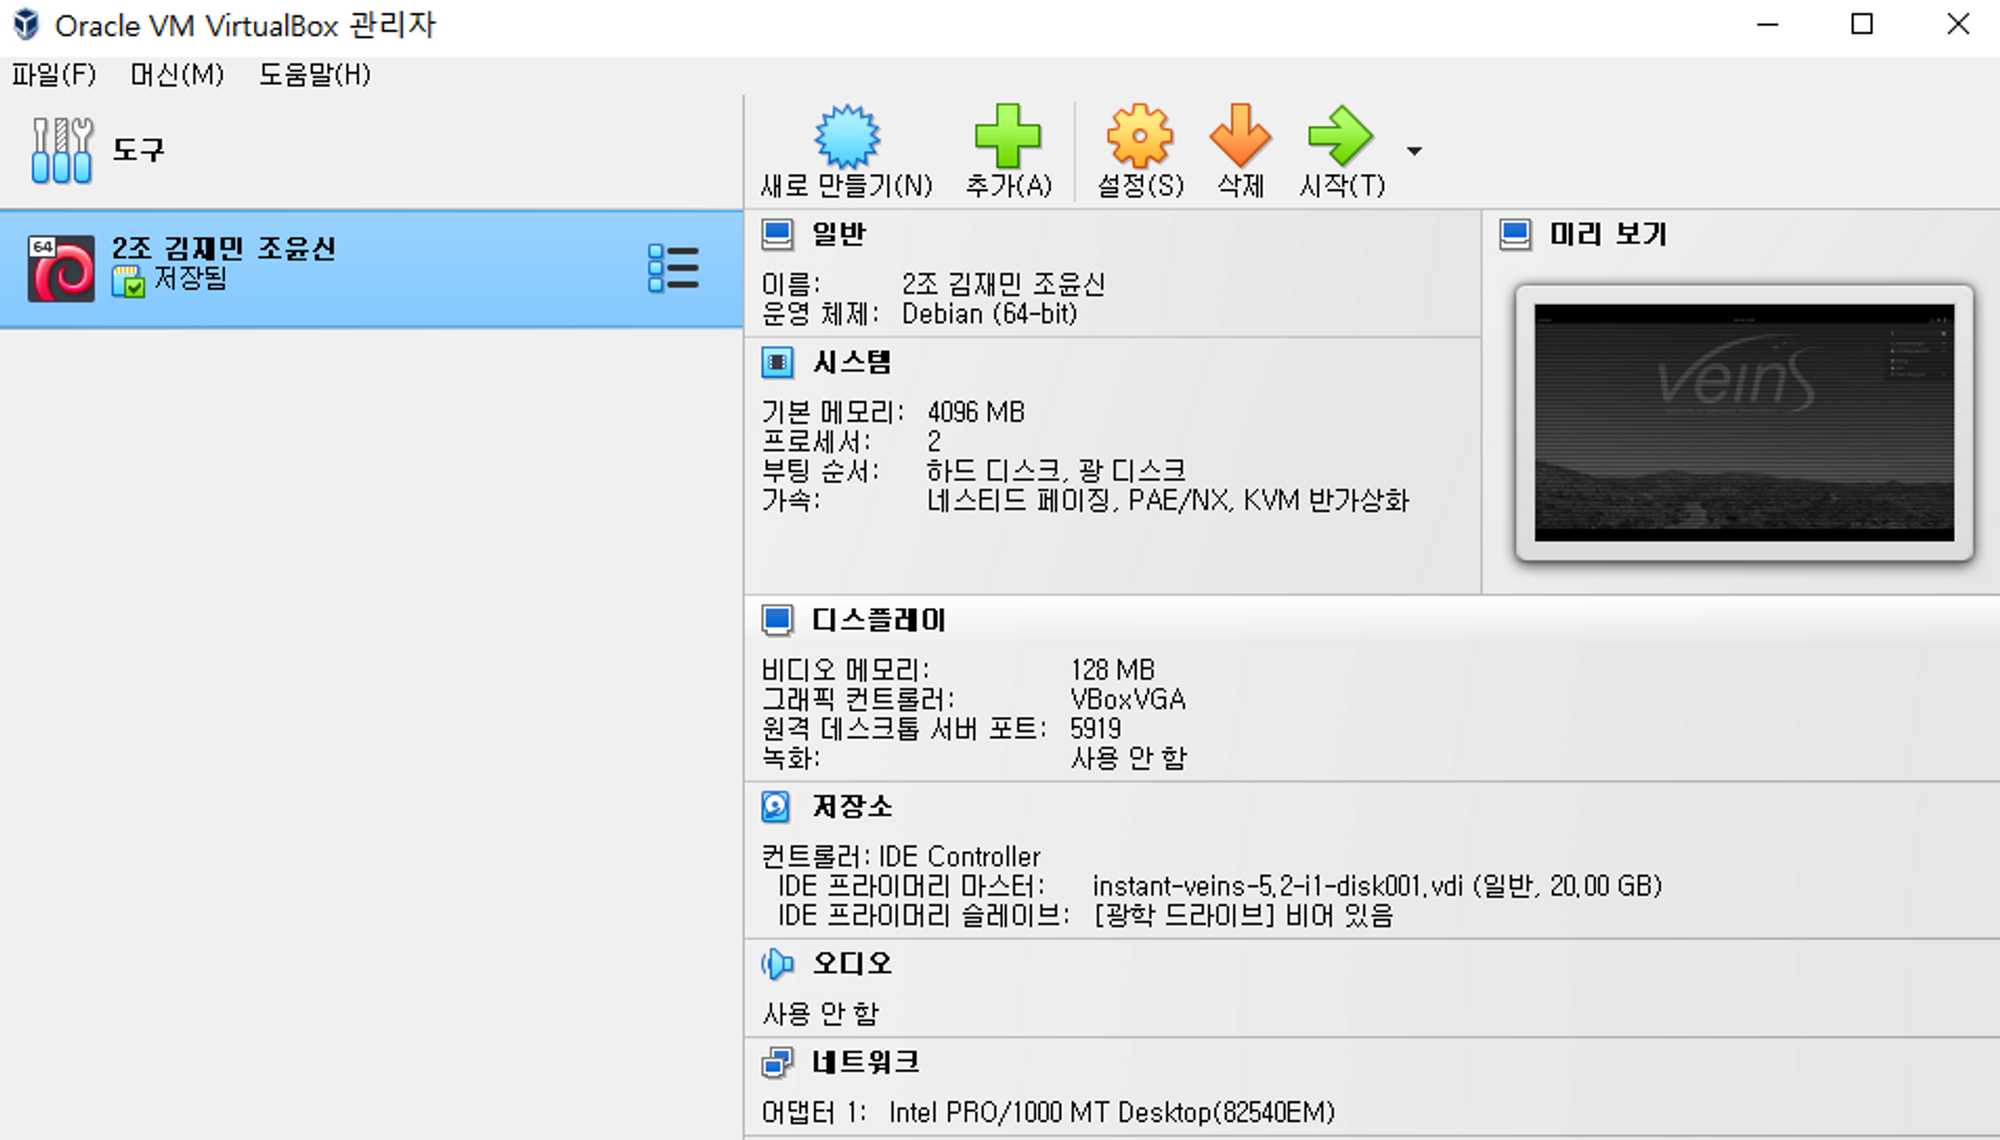
\includegraphics[width=.68\textwidth]{image/week13/0-1.png}
        \caption{\footnotesize
        Instant Veins virtual machine}
        \vspace{-10pt}
    \end{figure}
    
    sumo-launchd.py를 실행하여 OMNeT++와 SUMO 간 통신 연결을 프록시했다. 이후 OMNeT++를 실행하여 실험을 진행했다.
    \begin{figure}[!h]\centering 
        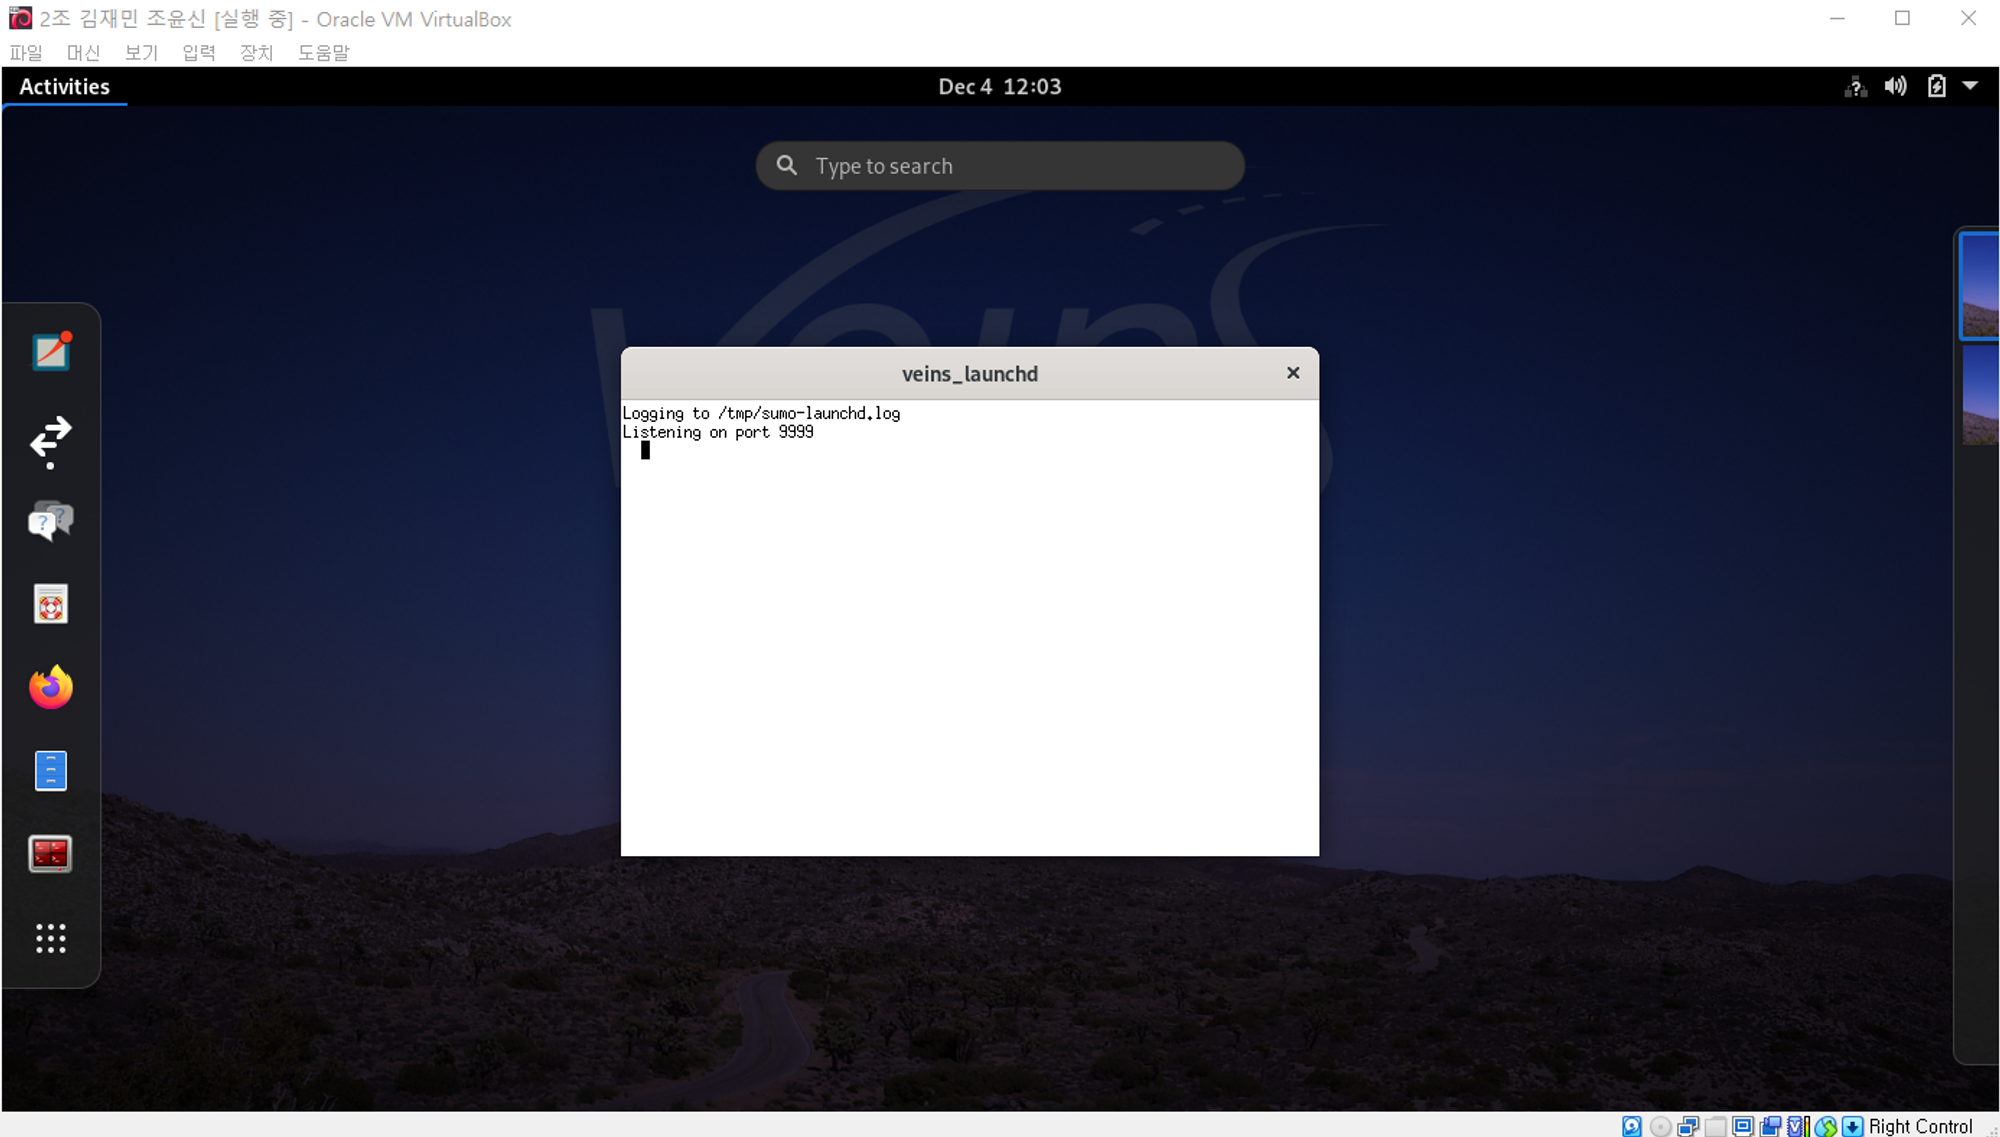
\includegraphics[width=.68\textwidth]{image/week13/0-2.png}
        \caption{\footnotesize
        sumo-launchd.py execution}
        \vspace{-10pt}
    \end{figure}
\newpage
    
%%%%%%%%%%%%%%%%%%%%%%%%%%%%%%%%%%%%%%%%%%%%%%%%%%%%%%%%%%%%%%%%%%%%%%%%%%%%%%%%%%%%%%%%%%%
    
\section*{Experiment 1 - VANET Tutorial}
    차량 한 대에 사고가 발생했을 때 , 사고 이후 Road Side Unit(RSU) 및 다른 차량 노드들 간 통신(V2I, V2V)을 통해 각 차량 노드들의 경로 상황을 분석하는 시뮬레이션이다. 
    
%%%%%%%%%%%%%%%%%%%%%%%%%%%%%%%%%%%%%%%%%%%%%%%%%%%%%%%%%%%%%%%%%%%%%%%%%%%%%%%%%%%%%%%%%%%
    
    \subsection*{Experiment 1-(a)}
        veins 내 기본 설정 값으로 시뮬레이션 진행한다.
        \subsubsection*{Simulation Results}
            RSU는 1개가 배치되어 있고 차량들은 우측 아래에서 3초 간격으로 출발한다. 첫 번째 차량은 출발 73초 후 50초간 사고가 발생한다. simulation 전체의 영상은 아래 링크를 클릭하여 확인할 수 있다.
            \vspace{-10mm}
                \begin{center}
                    \item \href{https://youtu.be/x1DFbwhNiEs}
        	        {Youtube link of Week13 Experiment 1-(a) Simulation Results Screenshot Video}
                \end{center}
            \vspace{-6mm}
            
            \begin{figure}[h!]
                \centering
                \subfloat{
                    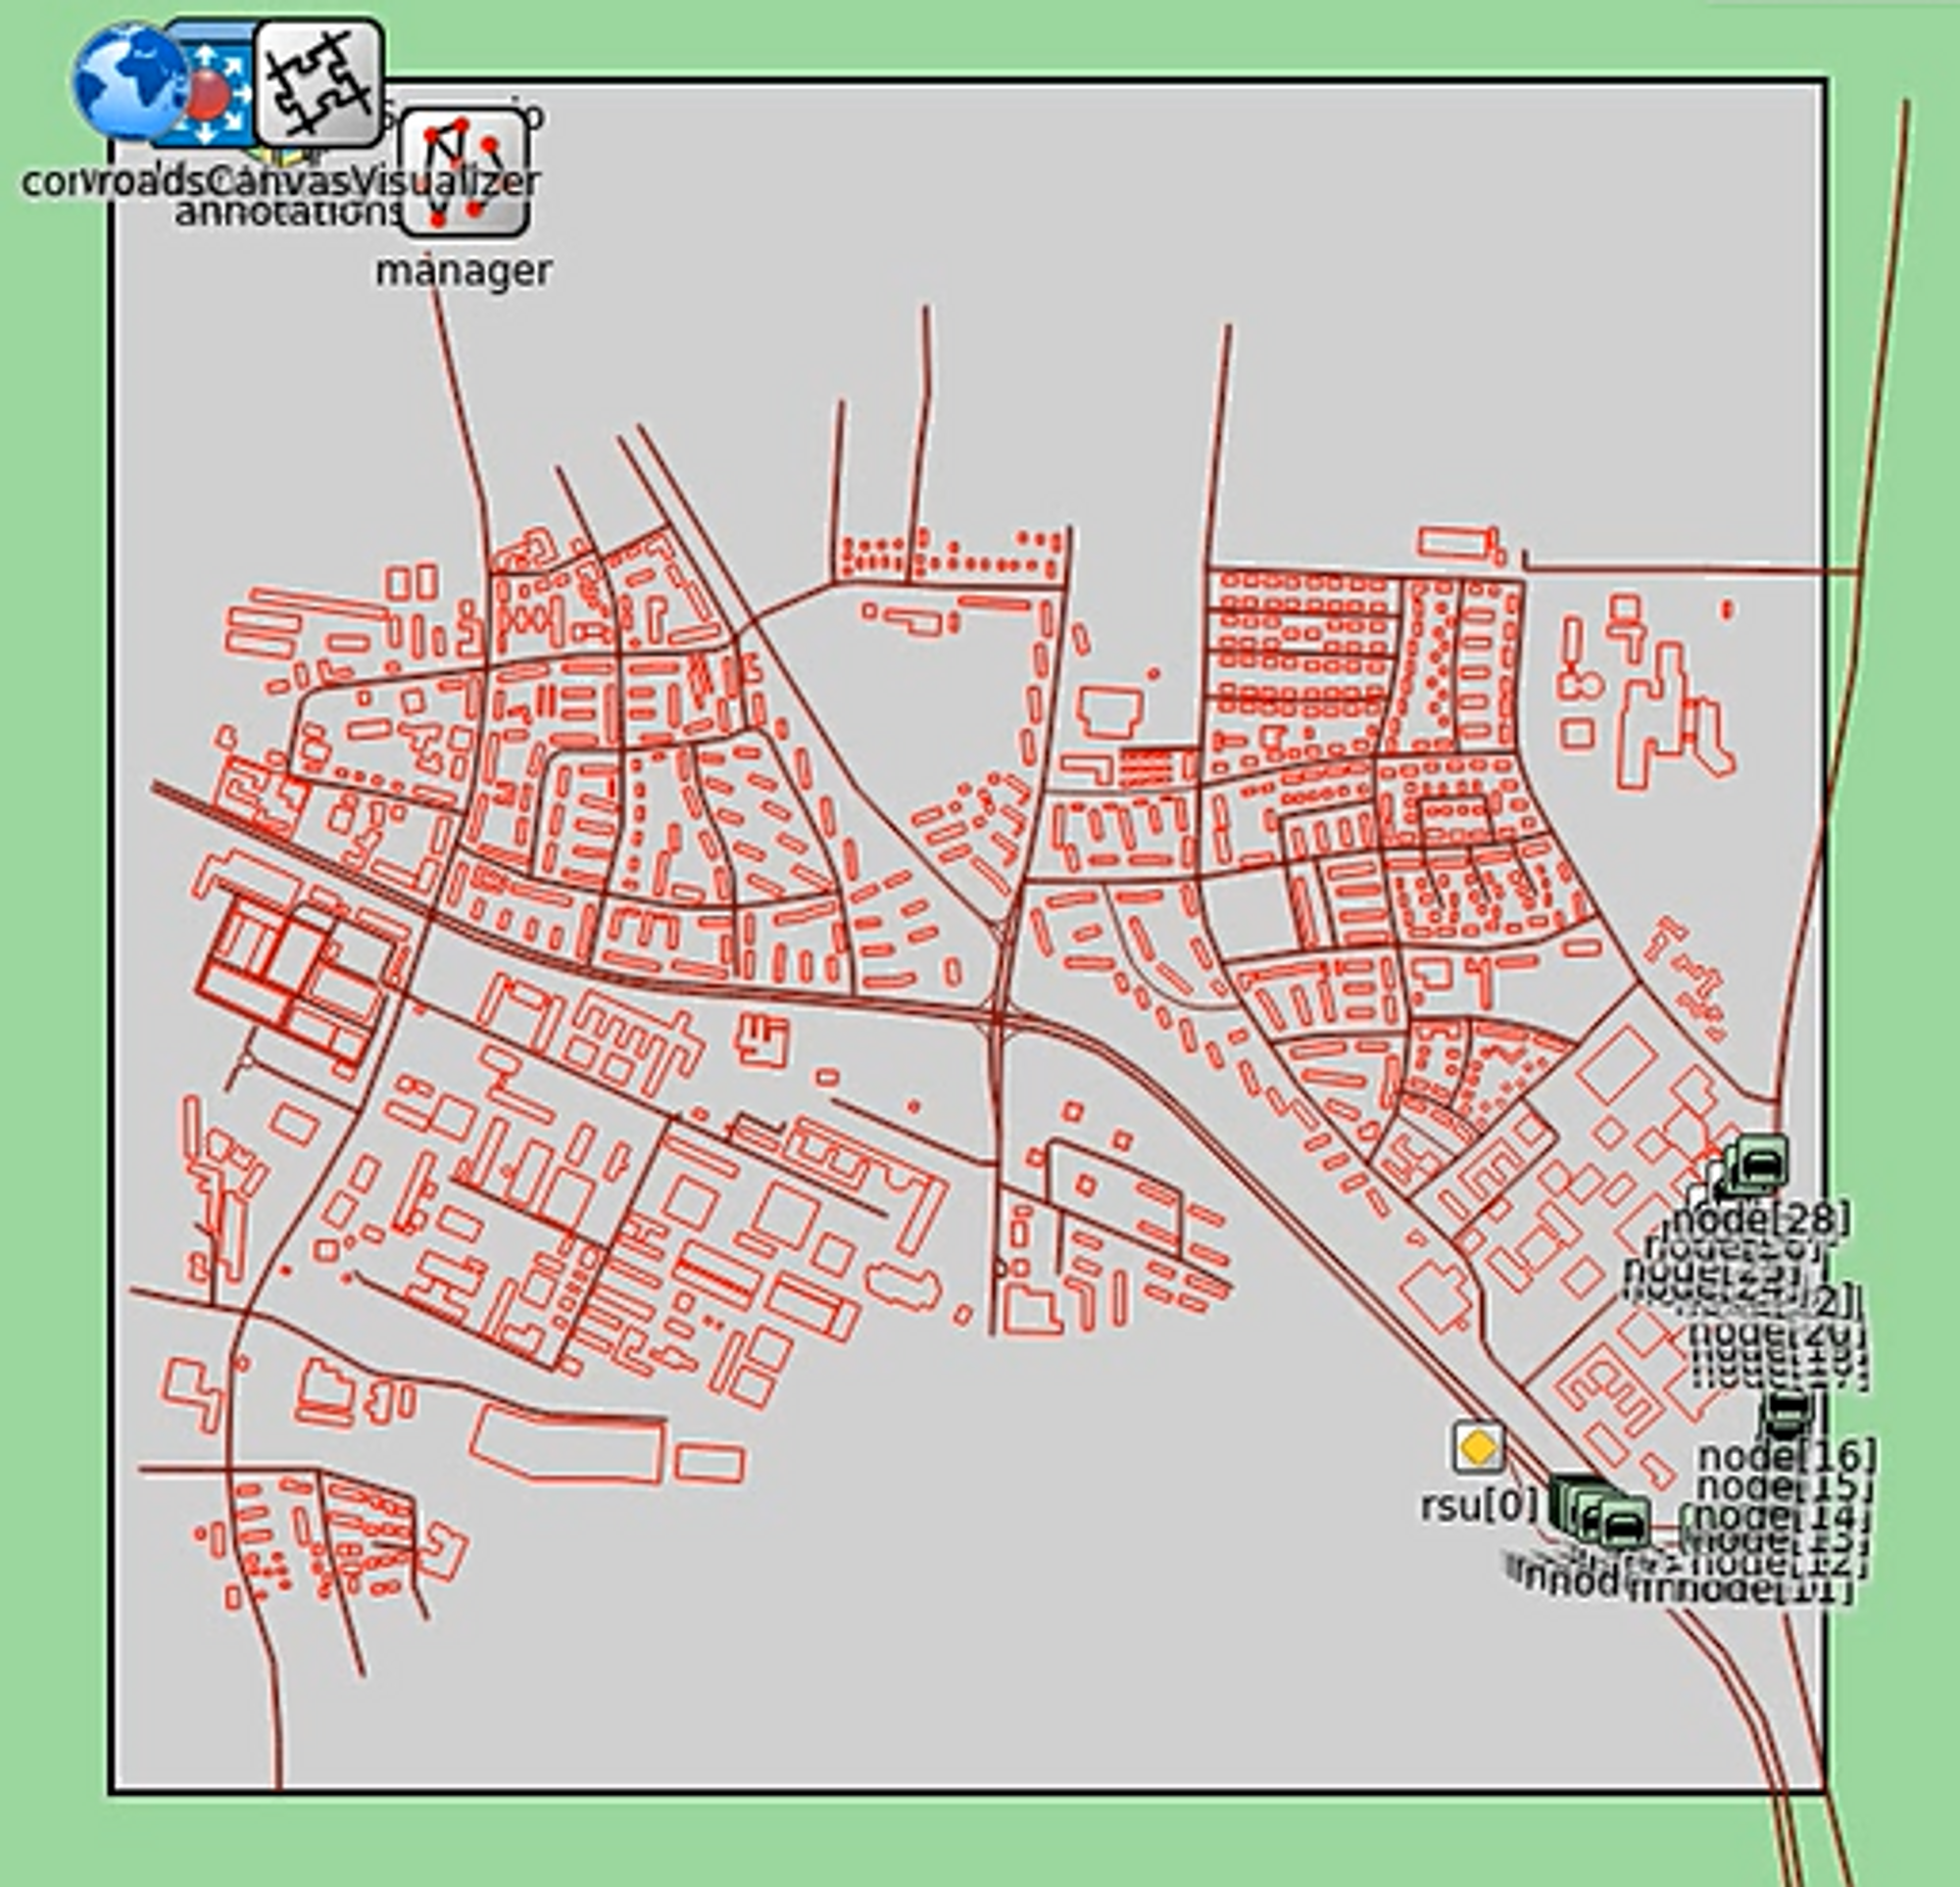
\includegraphics[width=0.46\textwidth]{image/week13/1-1.png}
                }\hspace{3mm}
                \subfloat{
                    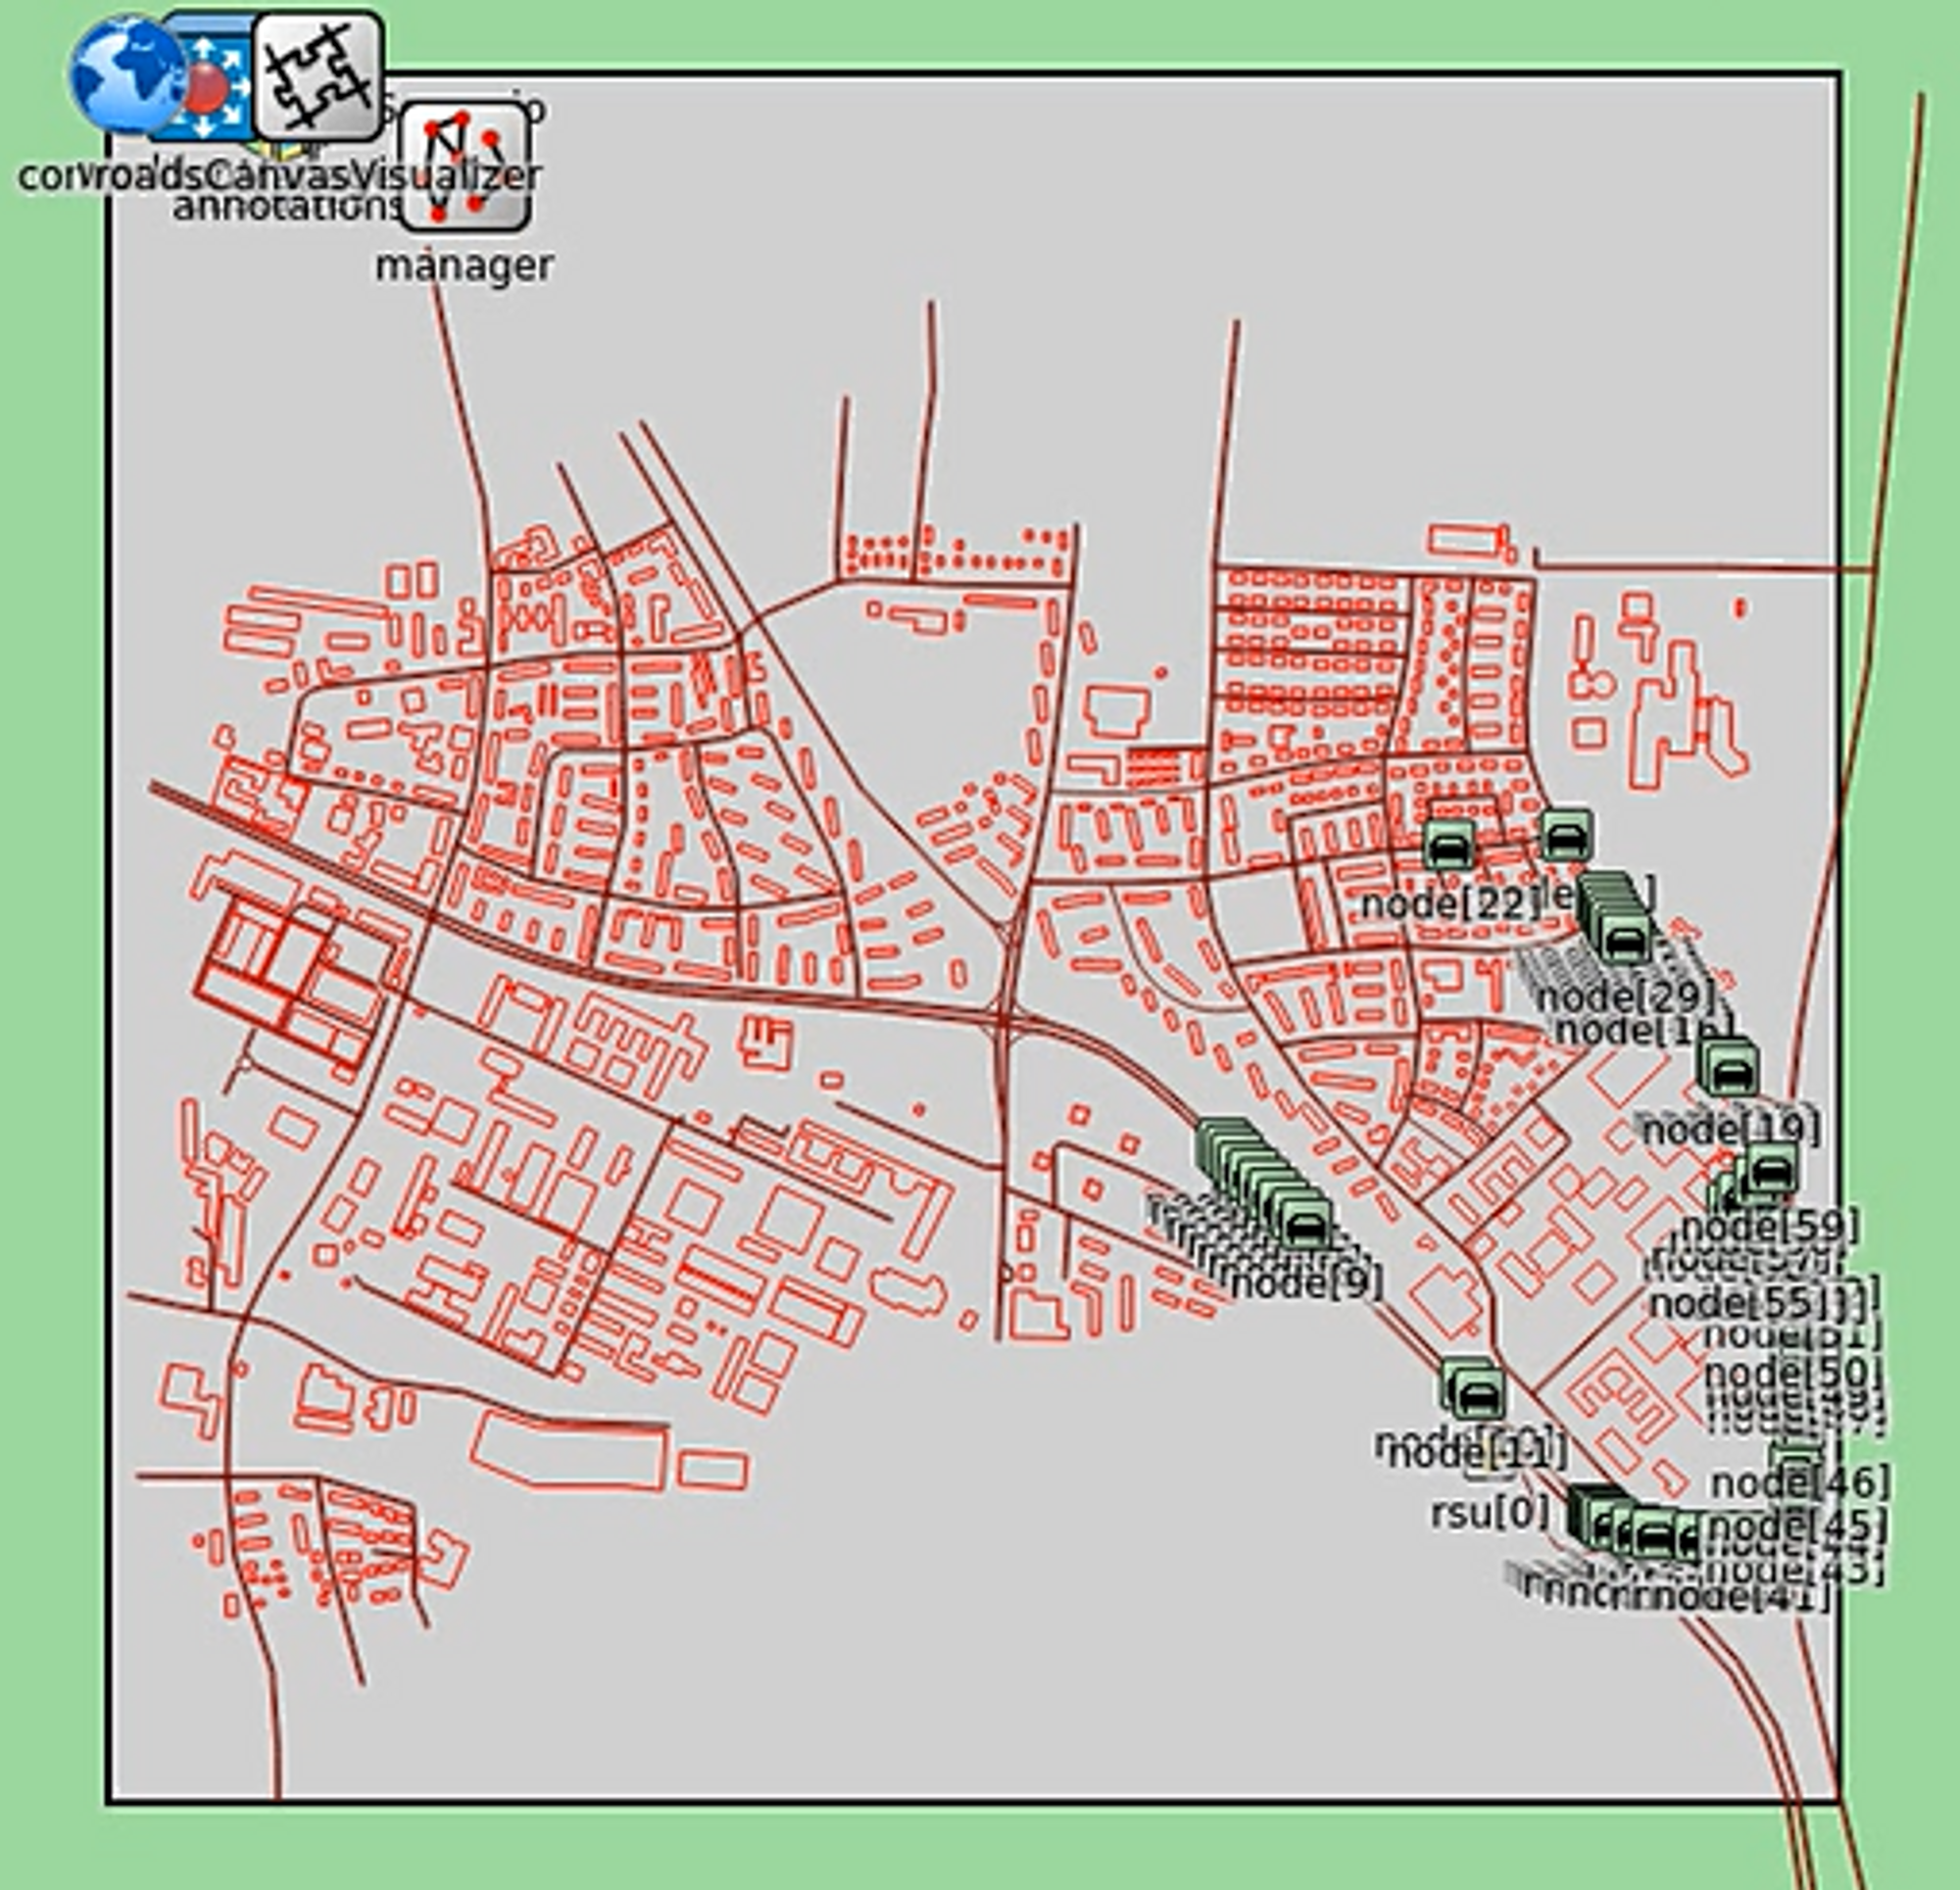
\includegraphics[width=0.46\textwidth]{image/week13/1-2.png}
                }
                \caption{Experiment 1-(a) Simulation Results Screenshot}
                \vspace{-2mm}
            \end{figure}
            
            시뮬레이션 종료 후 생성된 벡터 데이터 중에서 첫 번째 차량의 속도 그래프를 확인했다.
            \begin{figure}[!h]\centering 
                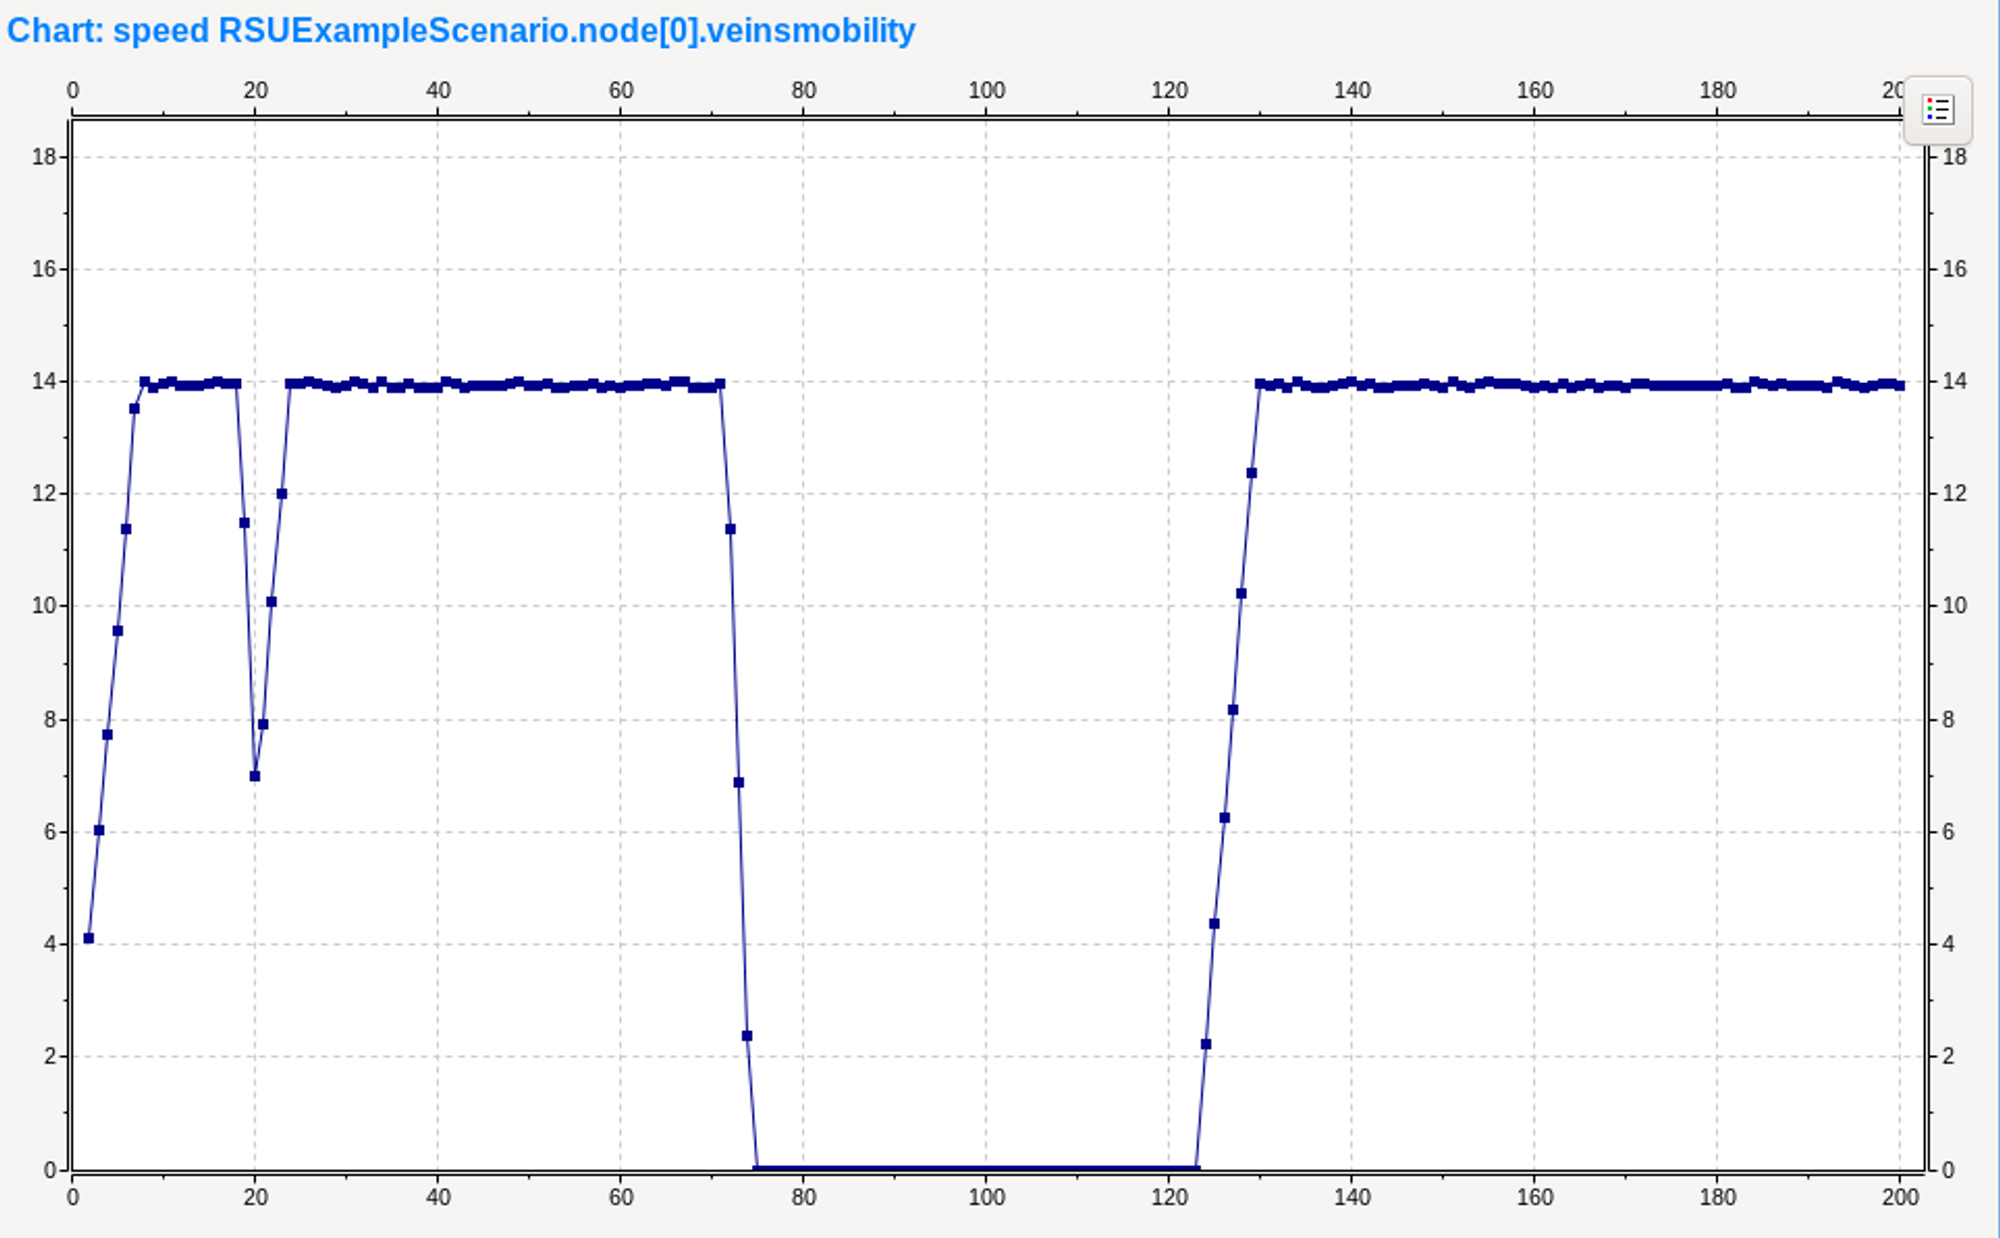
\includegraphics[width=.68\textwidth]{image/week13/1-3.png}
                \caption{\footnotesize
                1st vehicle speed graph}
                \vspace{-10pt}
            \end{figure}
            
        \subsubsection*{Discussion}
            시뮬레이션과 속도 그래프에서 확인할 수 있듯이, 첫번째 차량은 출발 73초 후 50초간 사고가 발생하여 정지한다. RSU와 차량 노드들이 교통 상황 정보를 송수신(V2I, V2V)하는 VANET을 형성한다. 첫 번째 차량으로부터 멀리 있는 차량들은 사고로 인해 교통이 안좋은 기존 경로가 아닌 위쪽 경로로 우회한다. \\
            아래의 그림은 RSU와 차량 노드들이 교통 상황 정보를 교환하는 장면이다.
            \begin{figure}[!h]\centering 
                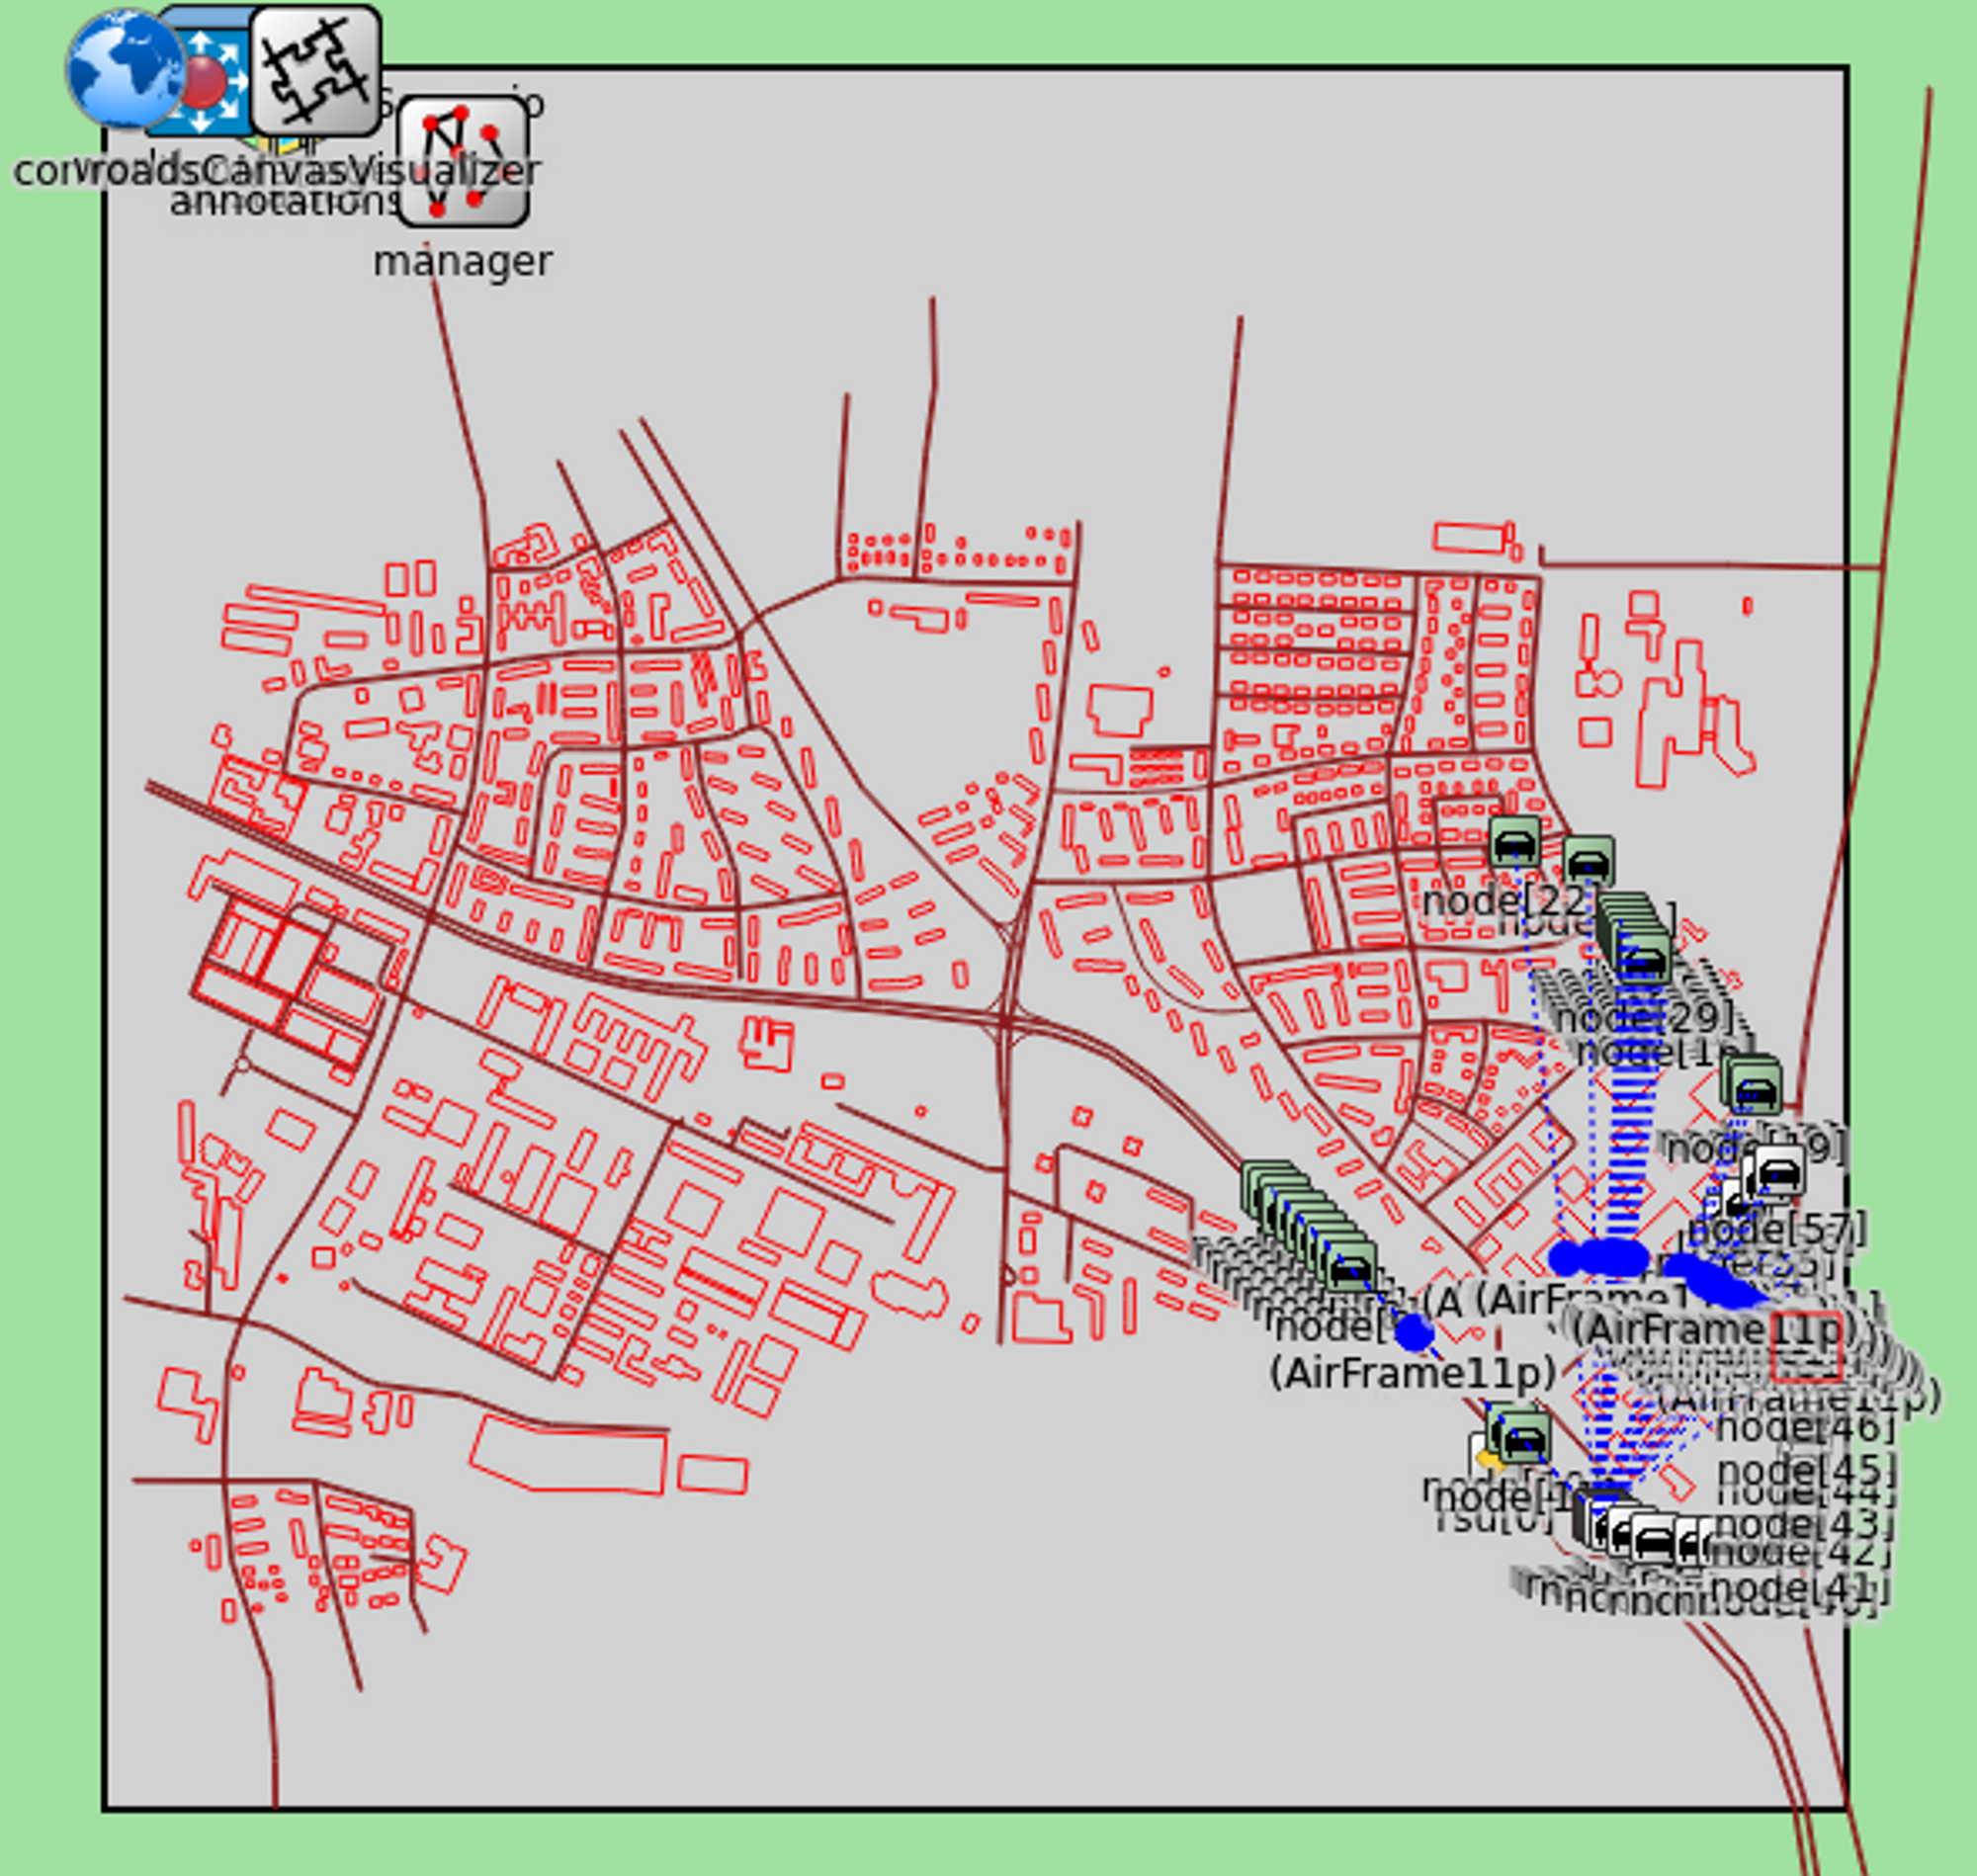
\includegraphics[width=.50\textwidth]{image/week13/1-4.png}
                \caption{\footnotesize
                Experiment 1-(a) VANET Communication}
                \vspace{-10pt}
            \end{figure}
\newpage
            
%%%%%%%%%%%%%%%%%%%%%%%%%%%%%%%%%%%%%%%%%%%%%%%%%%%%%%%%%%%%%%%%%%%%%%%%%%%%%%%%%%%%%%%%%%%

    \subsection*{Experiment 1-(b)}
        설정 값을 다음과 같이 바꾸어 시뮬레이션 진행한다.
        \begin{enumerate}
            \item 전체 시뮬레이션 시간을 300초로 설정한다.    \vspace{-1mm}
            \item RSU 2개를 각각 (1500, 1500), (1800, 1800)에 배치한다. \vspace{-1mm}
            \item 차량 노드 개수는 총 10개, 차량 노드 간 출발 간격은 20초로 설정한다. \vspace{-1mm}
            \item 첫 번째 차량 노드는 출발 50초 후 40초간, 5번째 차량 노도는 출발 80초 후 50초간 사고가 발생한다. \vspace{-1mm}
        \end{enumerate}
        
        \subsubsection*{Code Modified}
            veins 내 기본 설정에서 바꾼 부분의 코드이다.
            
            \textbf{omnetpp.ini}
            
            \vspace{-2mm}
            \begin{listing}[h!]
                \inputminted[framerule = 1pt,framesep = 2mm , frame = lines, fontsize=\scriptsize]{c}{./code/week13/omnetpp.cpp}
                \vspace{-3mm}
                \caption{\footnotesize omnetpp.ini}
                \vspace{-3mm}
            \end{listing}
            \vspace{-6mm}
            
            \textbf{Erlangen.rou.xml}
            
            \vspace{-2mm}
            \begin{listing}[h!]
                \inputminted[framerule = 1pt,framesep = 2mm , frame = lines, fontsize=\scriptsize]{c}{./code/week13/Erlangen.cpp}
                \vspace{-3mm}
                \caption{\footnotesize Erlangen.rou.xml}
                \vspace{-3mm}
            \end{listing}
            \vspace{-6mm}
            
            \textbf{RSUExampleScenario.ned}
            
            \vspace{-2mm}
            \begin{listing}[h!]
                \inputminted[framerule = 1pt,framesep = 2mm , frame = lines, fontsize=\scriptsize]{c}{./code/week13/RSU.cpp}
                \vspace{-3mm}
                \caption{\footnotesize RSUExampleScenario.ned}
                \vspace{-3mm}
            \end{listing}
            \vspace{-6mm}
            
        \subsubsection*{Simulation Results}
            RSU 2개가 배치되어 있고 10대의 차량들이 우측 아래에서 20초 간격으로 출발한다. 첫 번째 차량은 출발 50초 후 40초간, 5번째 차량 노도는 출발 80초 후 50초간 사고가 발생한다. simulation 전체의 영상은 아래 링크를 클릭하여 확인할 수 있다.
            \vspace{-10mm}
                \begin{center}
                    \item \href{https://youtu.be/NtHc8h8PbeE}
        	        {Youtube link of Week13 Experiment 1-(a) Simulation Results Screenshot Video}
                \end{center}
            \vspace{-6mm}
\newpage

            아래의 그림은 각각 100초, 200초, 300초 시점에서의 시뮬레이션 진행 화면이다.
            
            \begin{figure}[h!]
                \centering
                \subfloat[100s]{
                    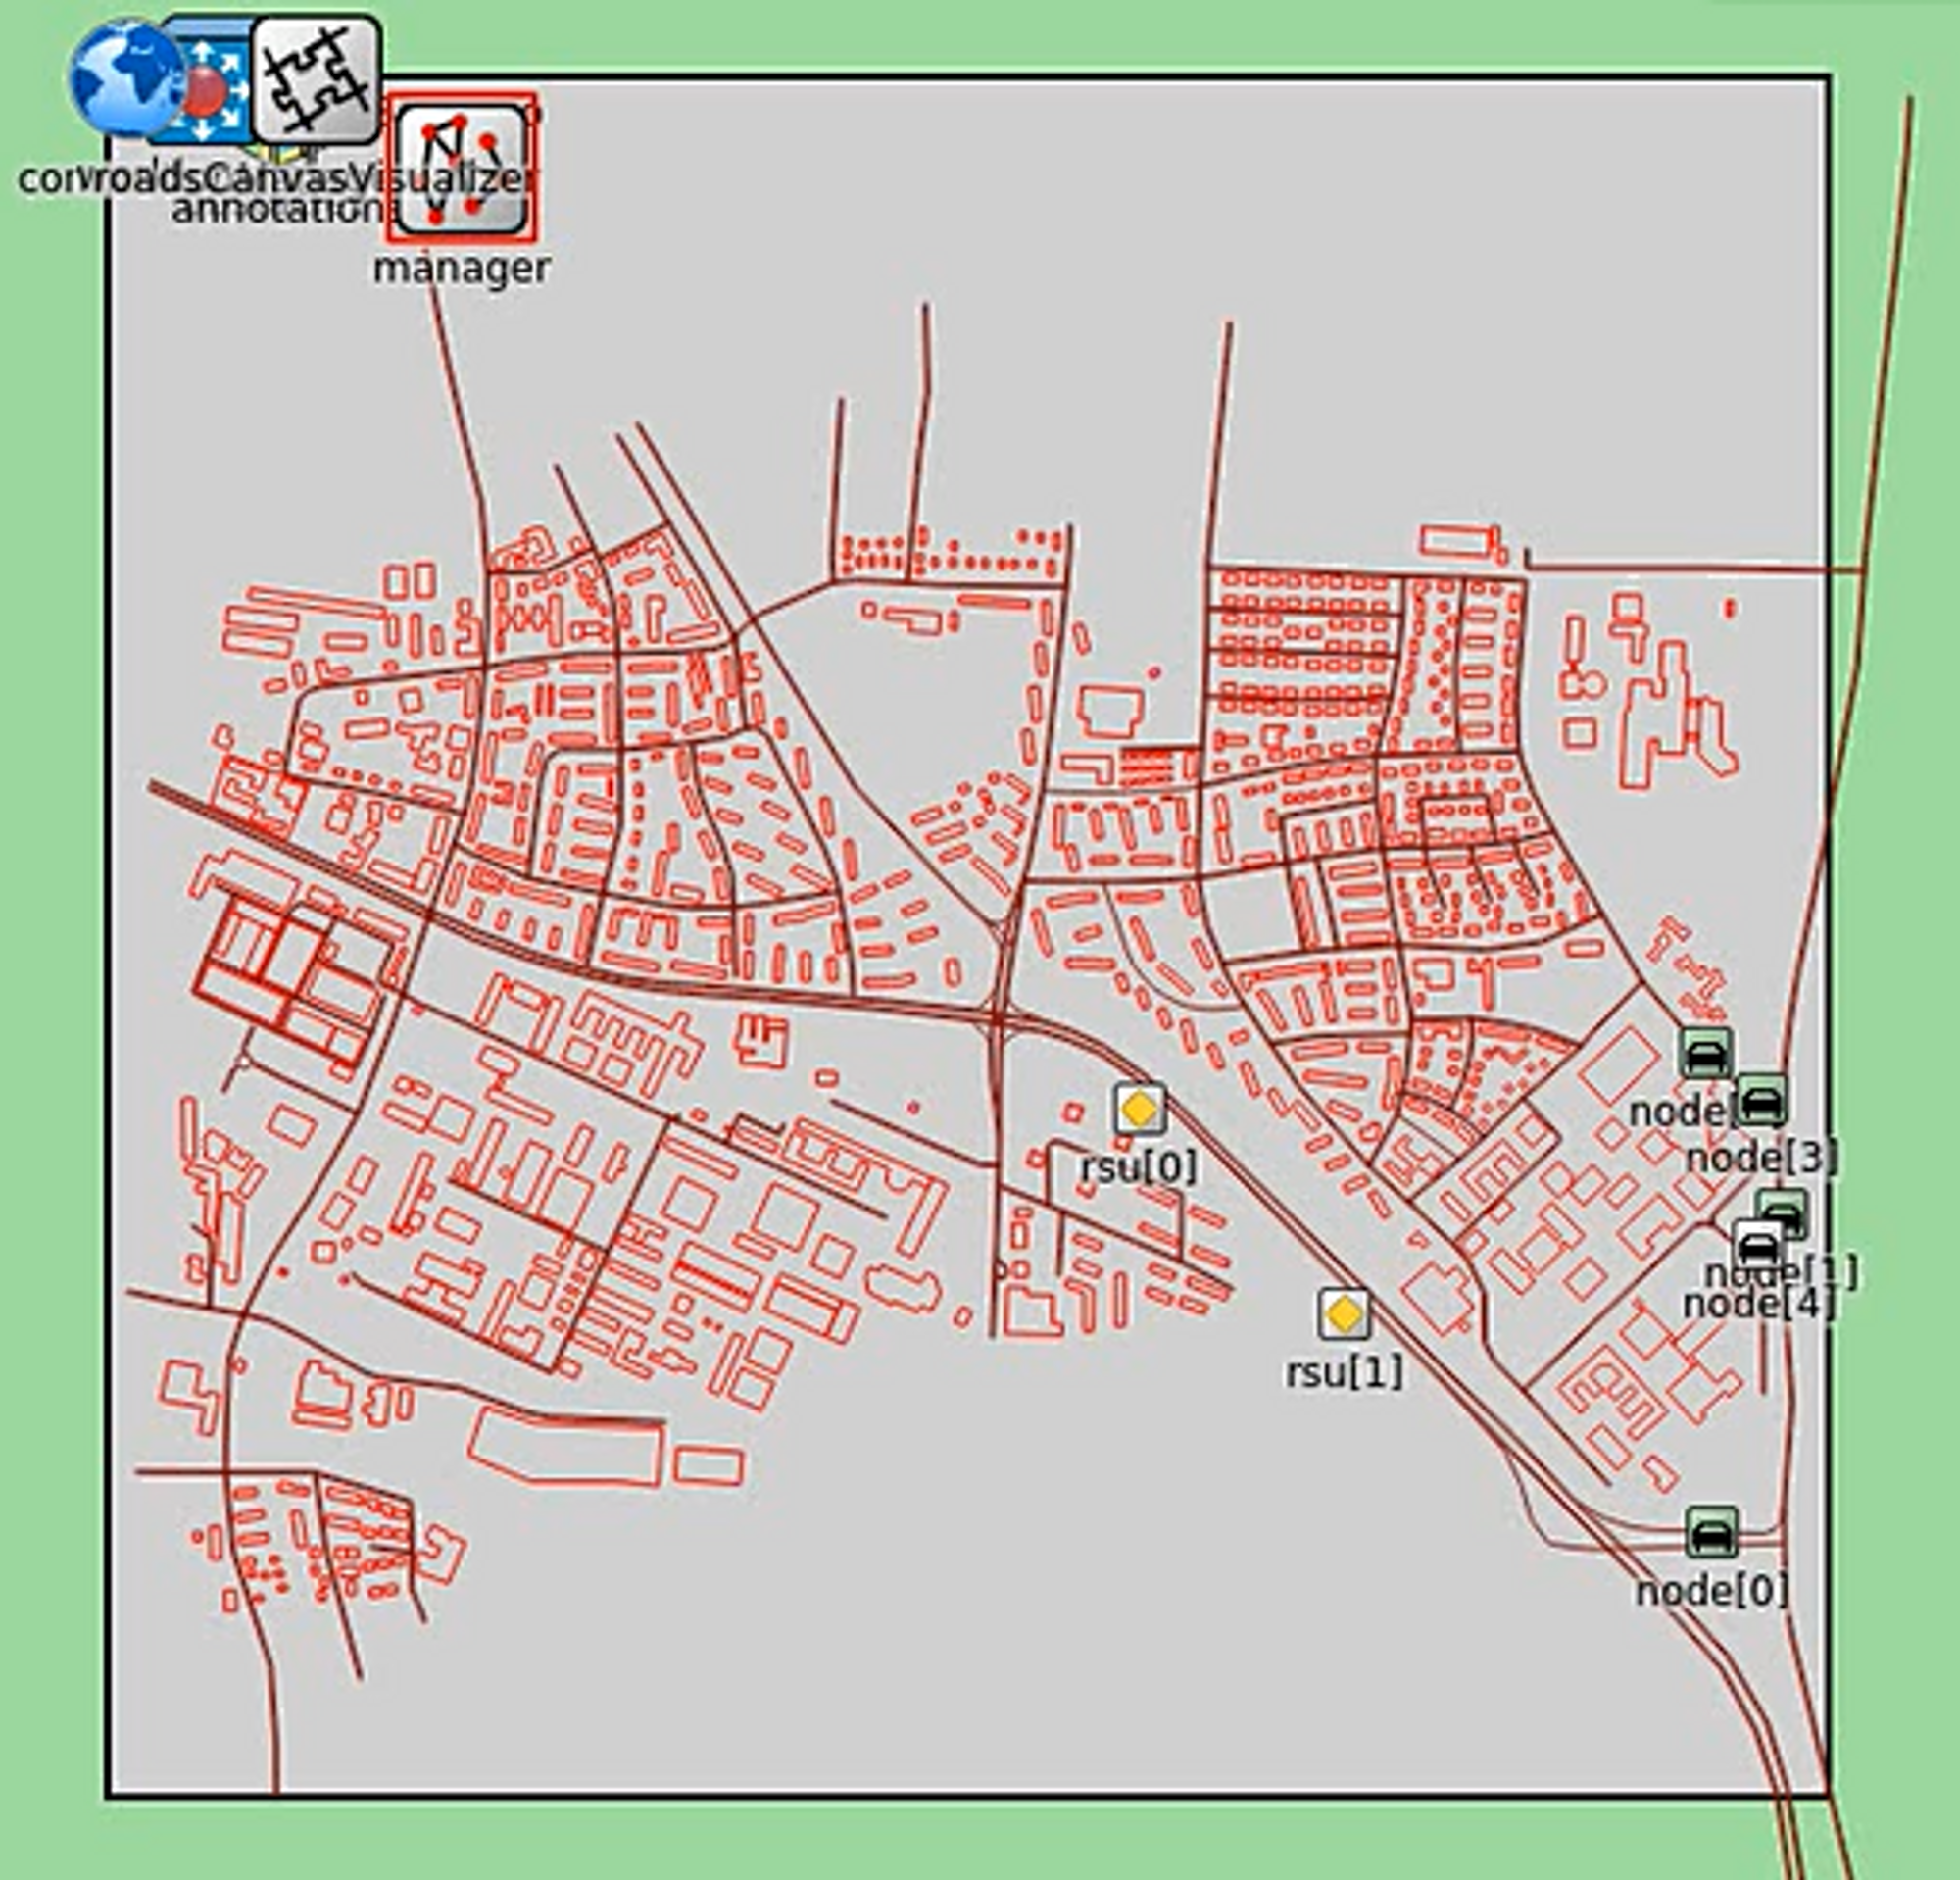
\includegraphics[width=0.46\textwidth]{image/week13/2-1.png}
                }\hspace{3mm}
                \subfloat[200s]{
                    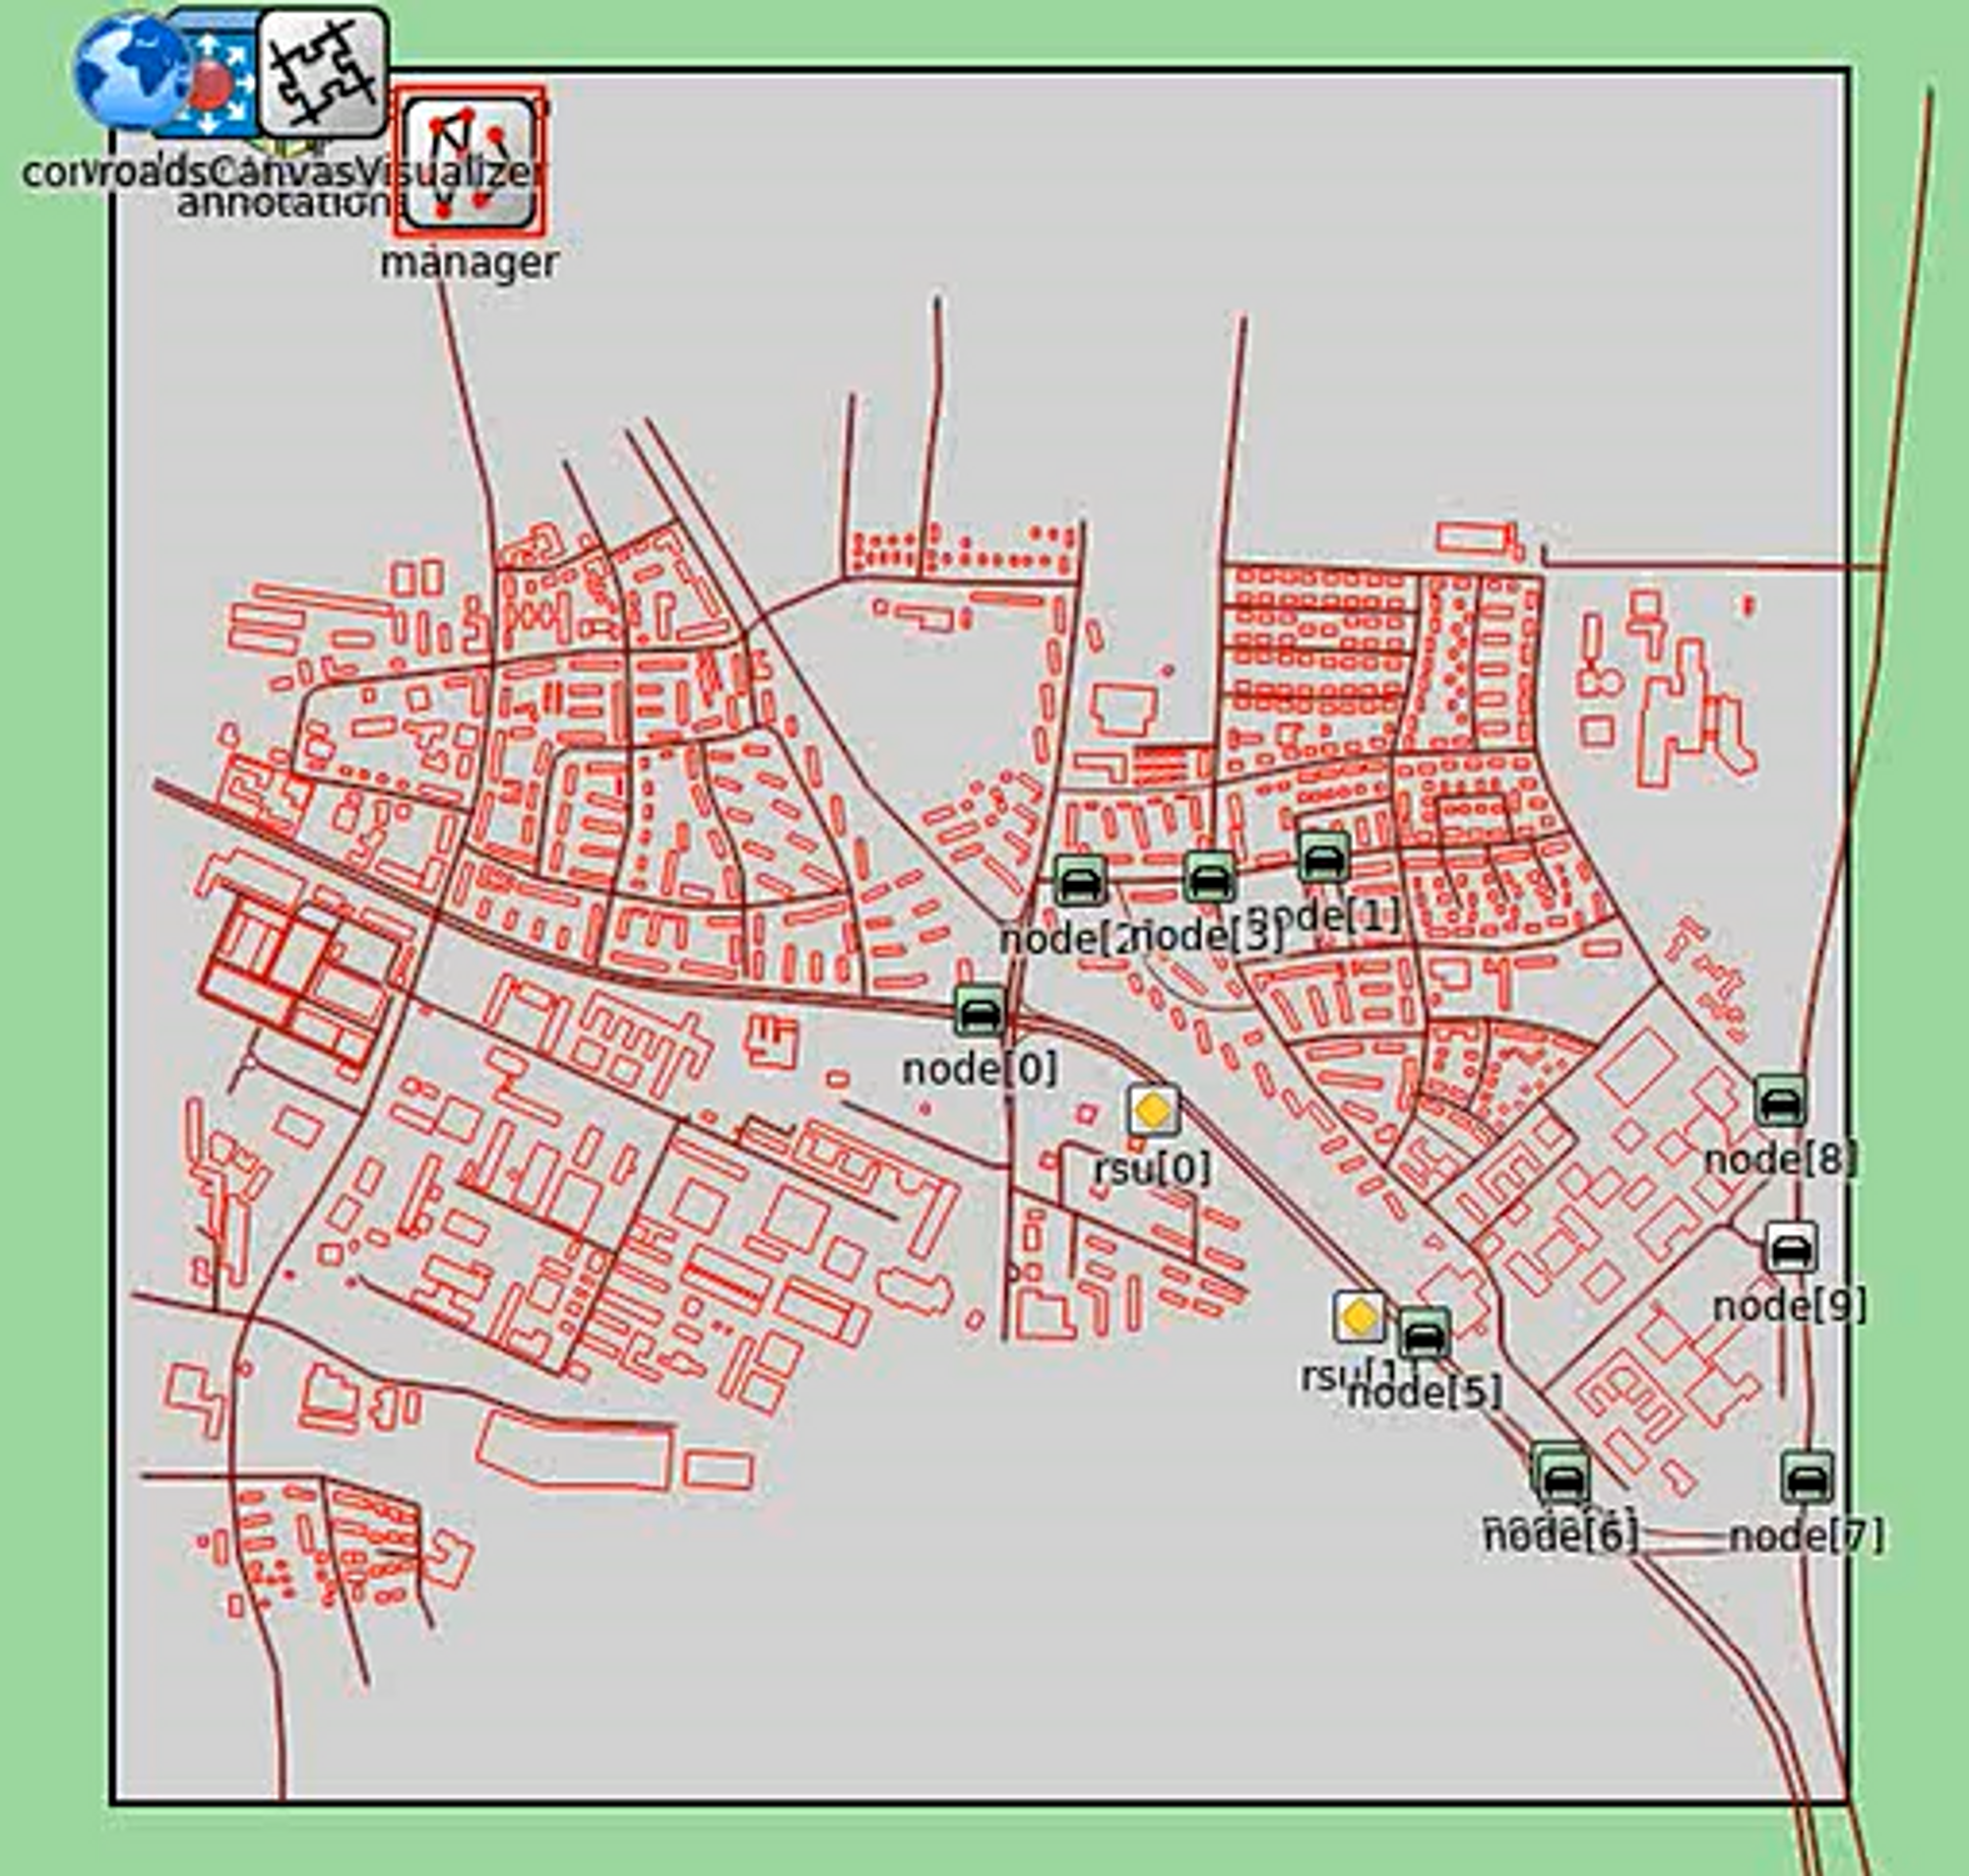
\includegraphics[width=0.46\textwidth]{image/week13/2-2.png}
                }
                \subfloat[300s]{
                    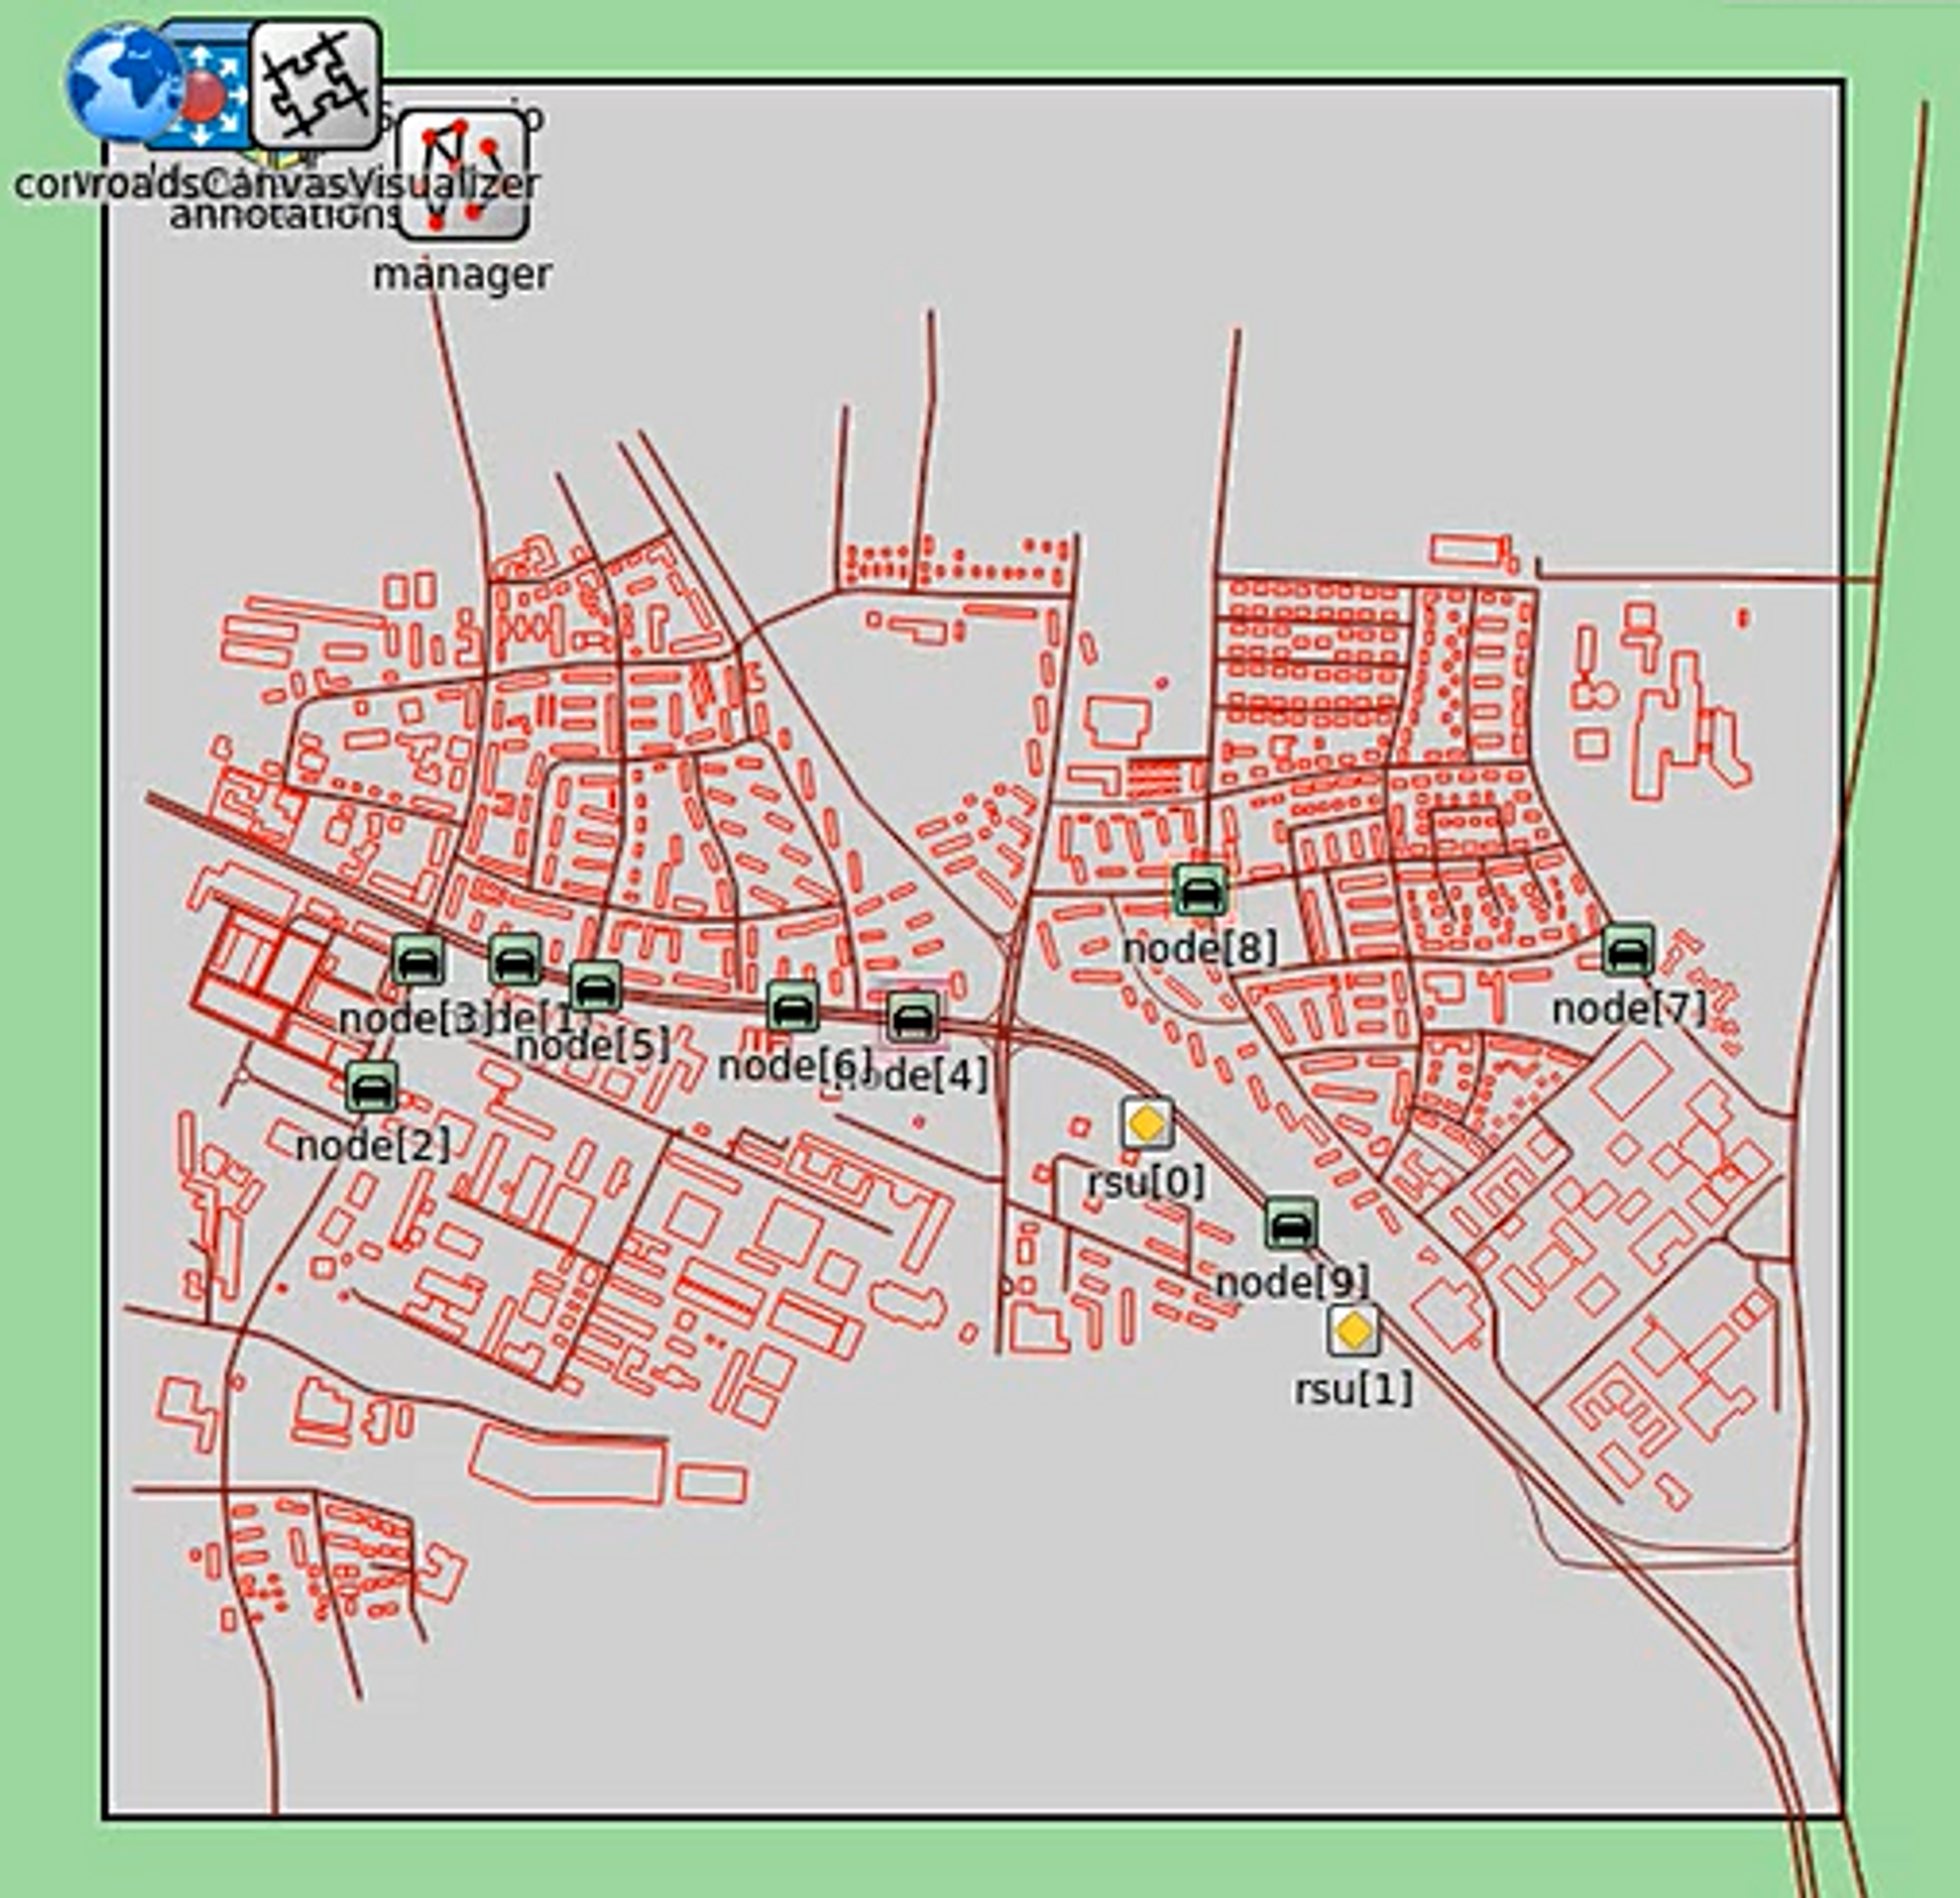
\includegraphics[width=0.46\textwidth]{image/week13/2-3.png}
                }
                \caption{Experiment 1-(b) Simulation Results Screenshot}
                \vspace{-2mm}
            \end{figure}
            
            시뮬레이션 종료 후 생성된 벡터 데이터 중에서 첫 번째 차량과 5번째 차량의 속도 그래프를 확인했다.
            \begin{figure}[h!]
                \centering
                \subfloat[1st vehicle]{
                    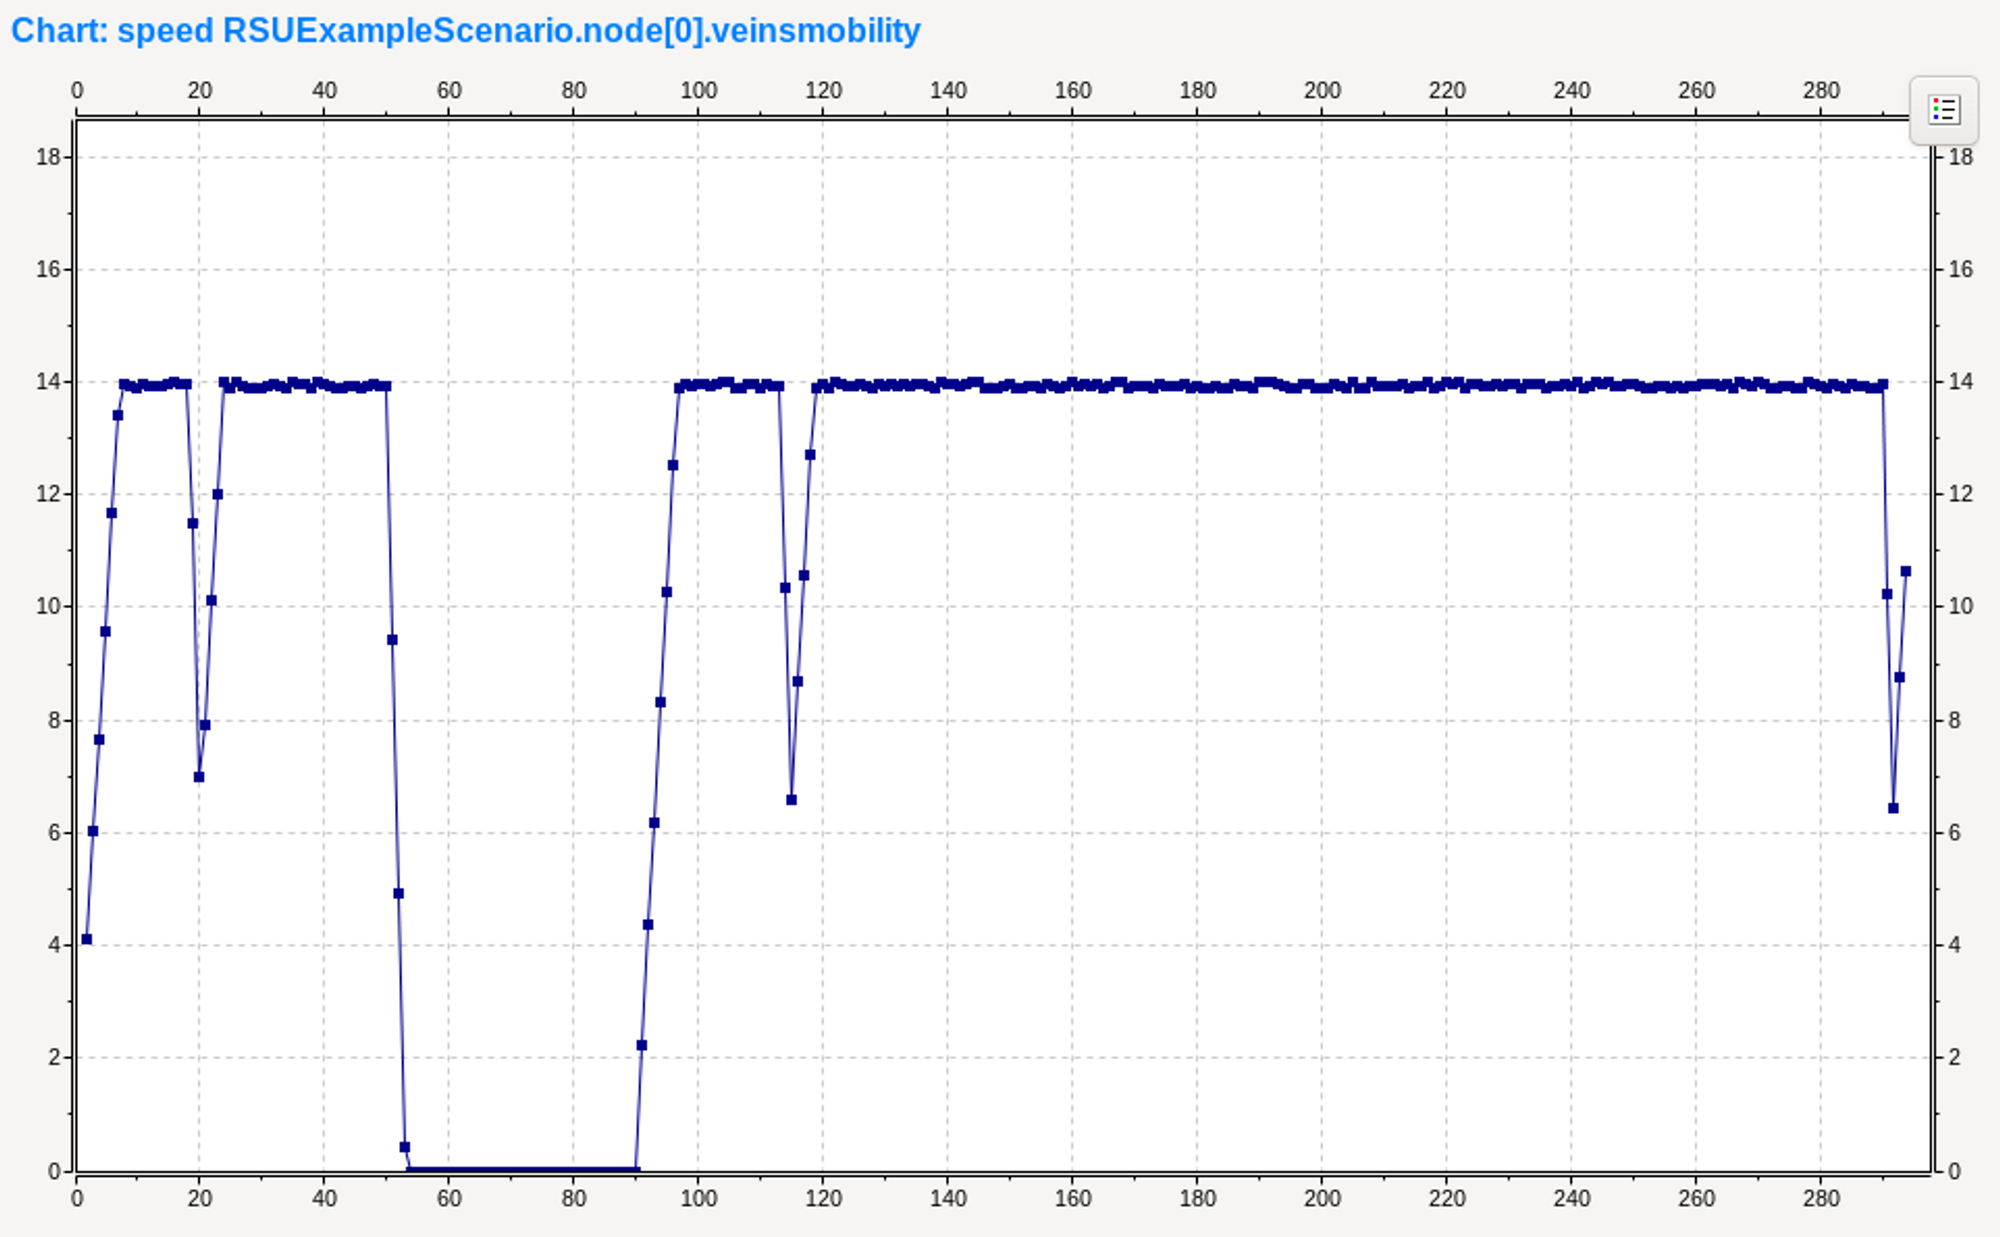
\includegraphics[width=0.46\textwidth]{image/week13/2-4.png}
                }\hspace{3mm}
                \subfloat[5th vehicle]{
                    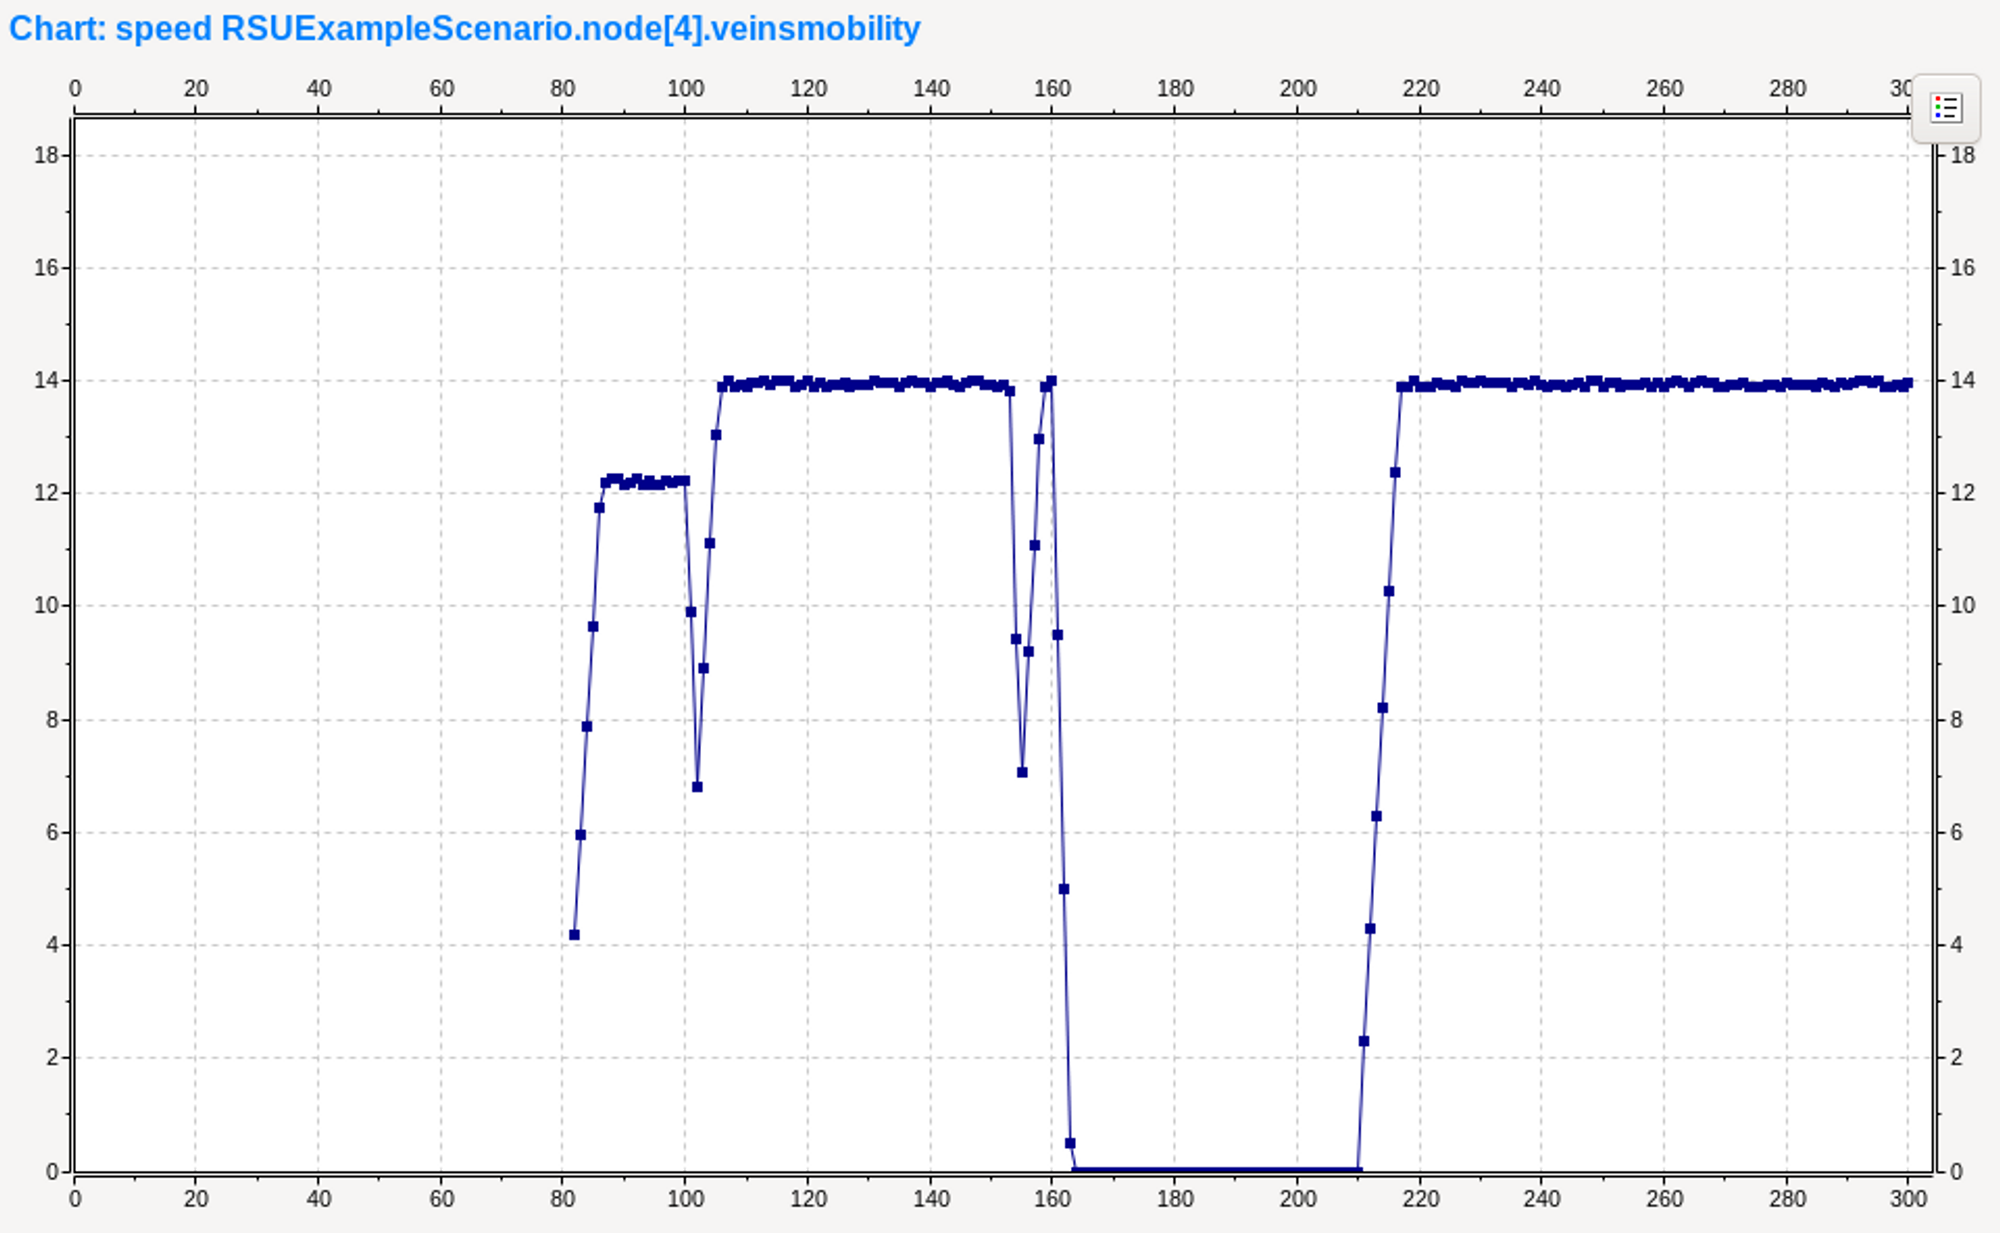
\includegraphics[width=0.46\textwidth]{image/week13/2-5.png}
                }
                \caption{Experiment 1-(b) 1st and 5th vehicles speed graph}
                \vspace{-2mm}
            \end{figure}
            
        \subsubsection*{Discussion}
            첫번째 차량은 출발 50초 후 40초간 사고가 발생하여 정지한다. RSU와 차량 노드들이 교통 상황 정보를 송수신(V2I, V2V)하는 VANET을 형성한다. 사고가 발생한 첫 번째 차량을 뒤따라 오는 2, 3, 4번째 차량은 사고로 인해 교통이 안좋은 기존 경로가 아닌 위쪽 경로로 우회한다. \\
            5번째 차량은 출발 80초 후(160초) 50초간 사고가 발생하여 정지한다. 5번째 차량으로부터 멀리 있는 8, 9번째 차량은 사고로 인해 교통이 안좋은 기존 경로가 아닌 위쪽 경로로 우회한다. \\
            아래의 그림은 RSU와 차량 노드들이 교통 상황 정보를 교환하는 장면이다. \\
            \begin{figure}[!h]\centering 
                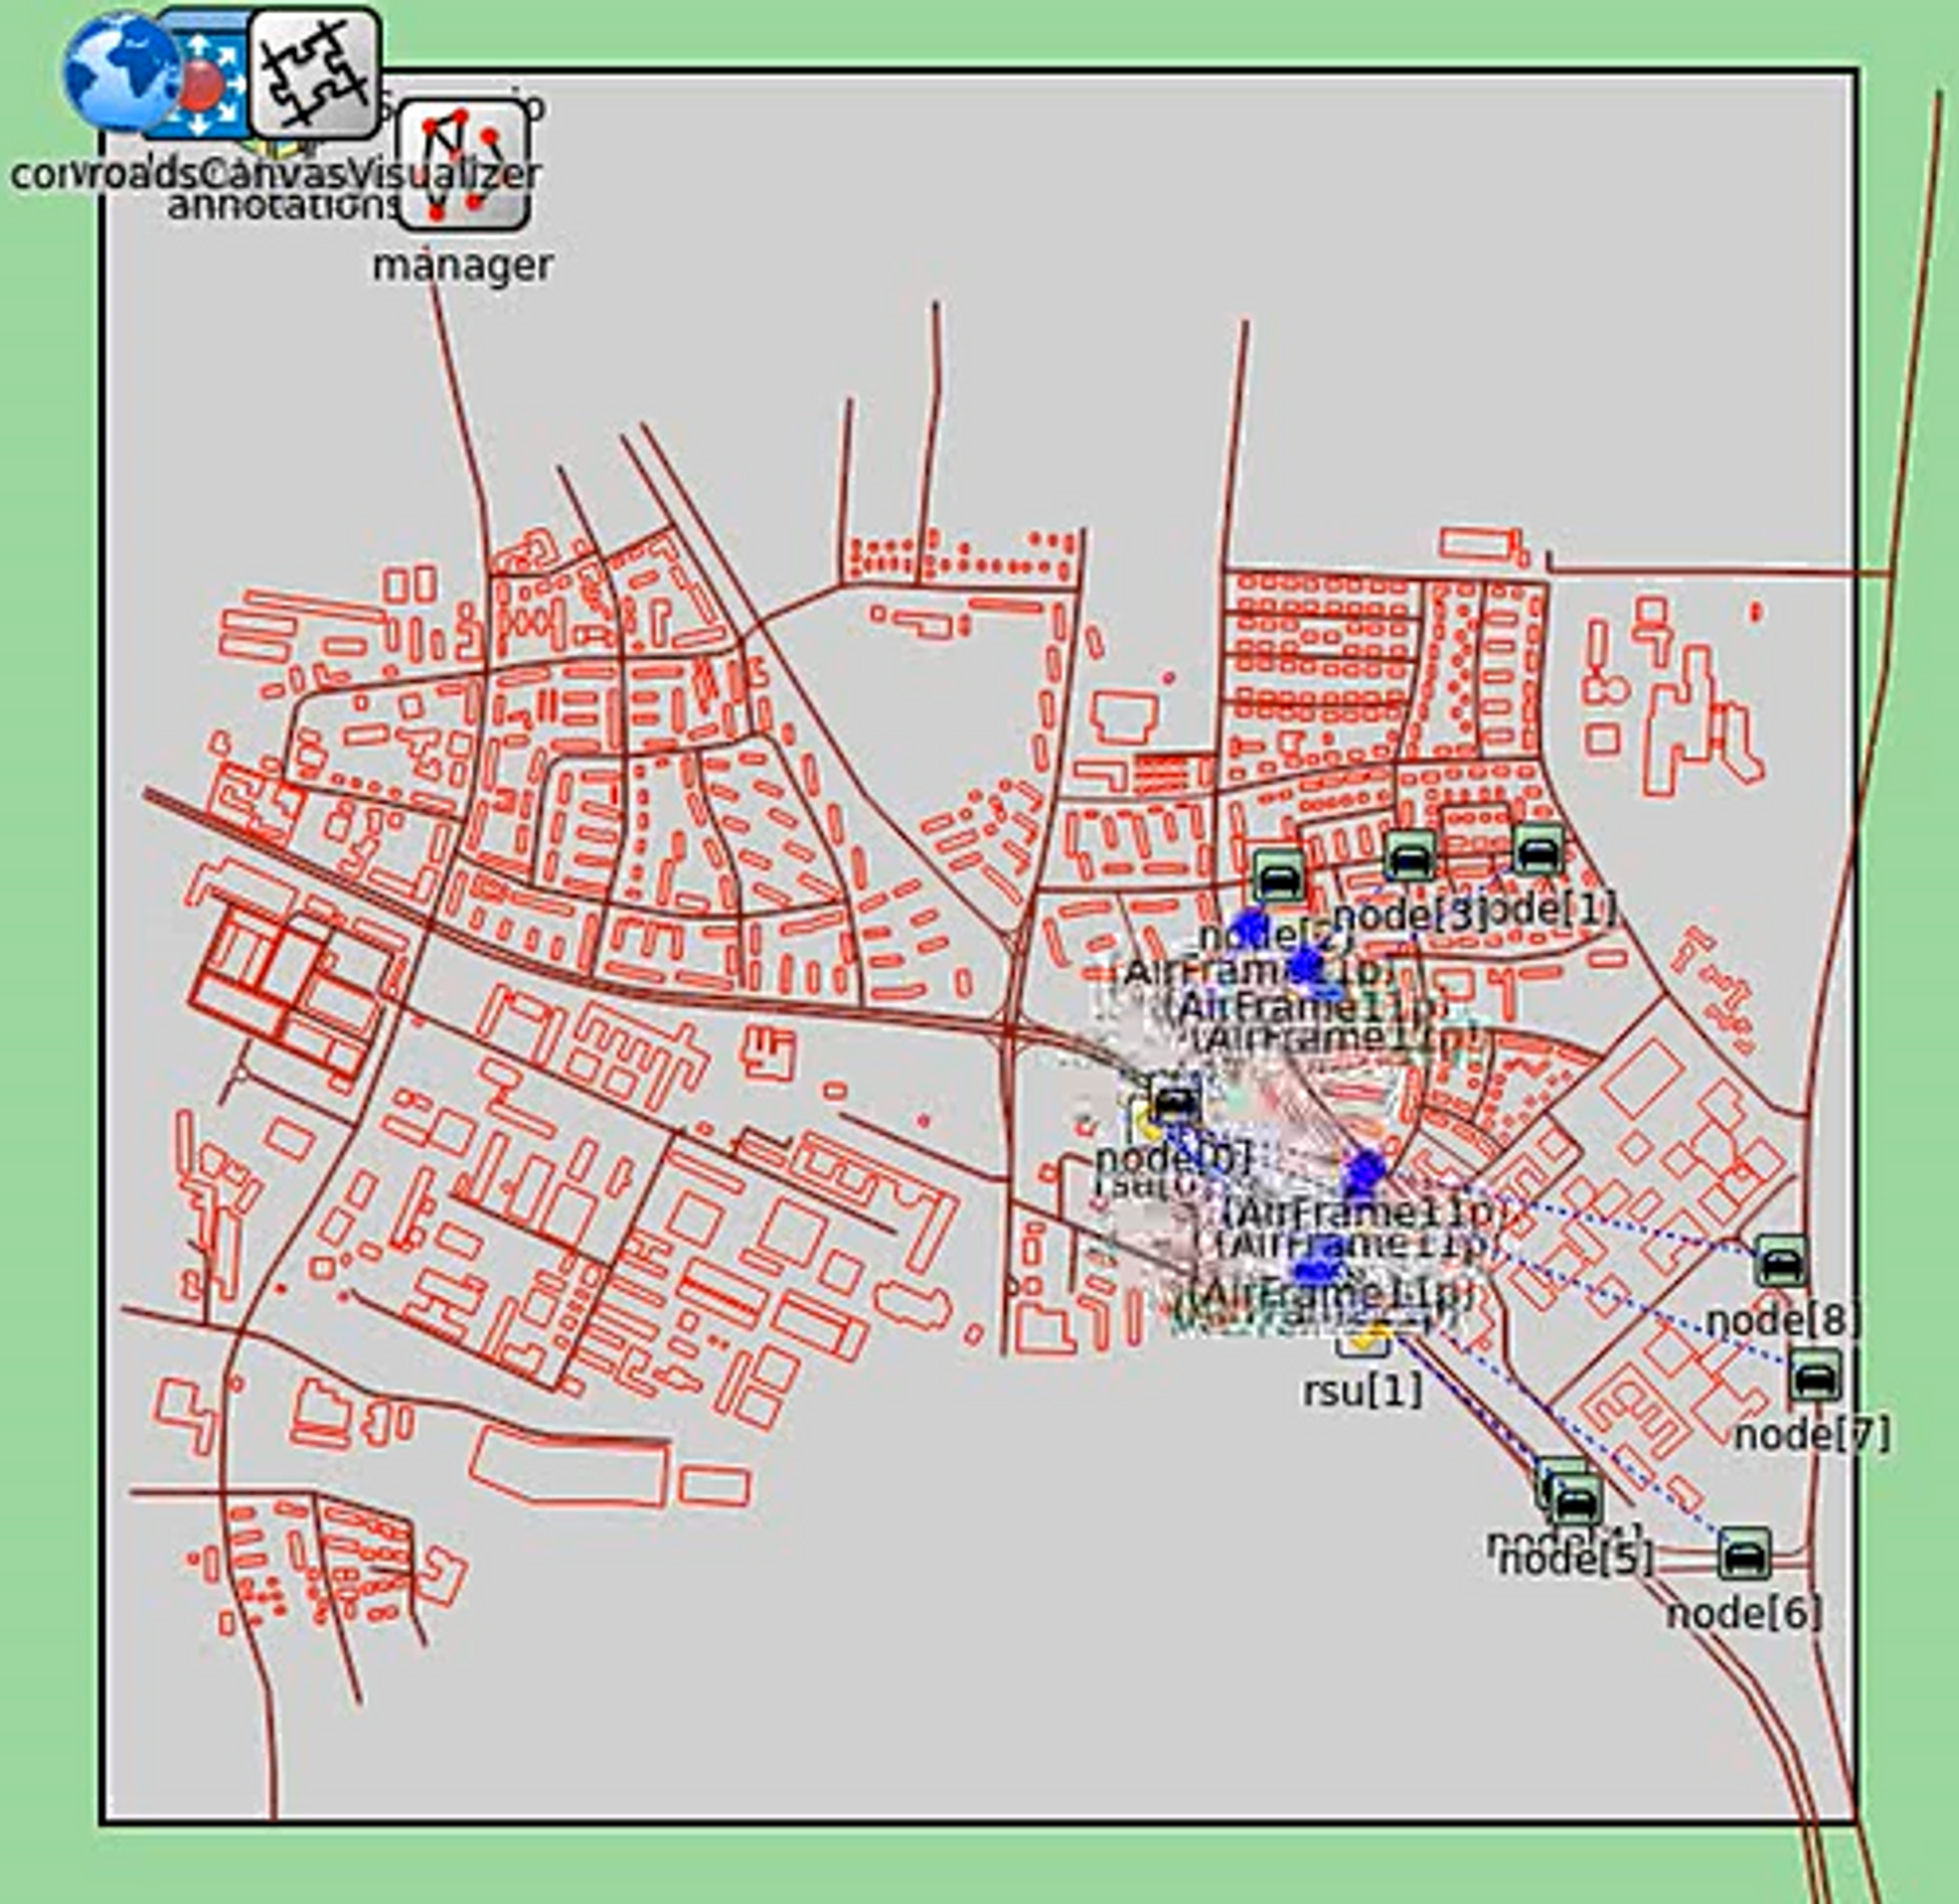
\includegraphics[width=.50\textwidth]{image/week13/2-6.png}
                \caption{\footnotesize
                Experiment 1-(b) VANET Communication}
                \vspace{-10pt}
            \end{figure}